% !Mode:: "TeX:UTF-8"
%% !TEX program  = xelatex
%! TEX program = xelatex
%\documentclass{cumcmthesis}
\documentclass[withoutpreface,bwprint]{cumcmthesis} %去掉封面与编号页,电子版提交的时候使用。

\usepackage{etoolbox}
\BeforeBeginEnvironment{tabular}{\zihao{-5}}
\usepackage{cite}
\usepackage[numbers,sort&compress]{natbib}
\usepackage[framemethod=TikZ]{mdframed}
\usepackage{url}   % 网页链接
\usepackage{subcaption} % 子标题
\title{基于逐步迭代方法的FAST节点调节优化}
\tihao{A}
\baominghao{4321}
\schoolname{华中科技大学}
\membera{ }
\memberb{ }
\memberc{ }
\supervisor{ }
\yearinput{2020}
\monthinput{08}
\dayinput{22}
\usepackage{yhmath}
\graphicspath{{figures/}}

%\usepackage{enumerate}
%\usepackage{graphicx}
%\setlength{\leftmargin}{1.2em} %左边界
%\setlength{\parsep}{0ex} %段落间距
%\setlength{\topsep}{1ex} %列表到上下文的垂直距离
%\setlength{\itemsep}{0.5ex} %条目间距
%\setlength{\labelsep}{0.3em} %标号和列表项之间的距离,默认0.5em
%\setlength{\itemindent}{1.5em} %标签缩进量
%\setlength{\listparindent}{0em} %段落缩进量




\begin{document}
	\graphicspath{{figures/}}
	\maketitle
	\begin{abstract}
	FAST望远镜通过调节反射曲面拟合抛物面,以提高观测精度,理想抛物面的选取与节点调节算法关系到拟合精度,本文基于黄金分割法与迭代优化建立了反射平面调节与评估的数学模型。
	
	\textbf{对于问题一},通过二维投影与极坐标建立简化抛物面方程,并集中优化参数到抛物面顶点偏移量h,以节点最小径向移动距离为目标,设置步长试探得到偏移量与移动距离的关系,在可调节区间内呈\textbf{单下峰函数}。再利用\textbf{黄金分割法}逐步缩小区间,逼近极小值点,精度设置为0.0001,求得最优解$\bm{h=0.4444m}$,据此确定抛物线方程$\bm{x^{2} + y^{2} =2\times280.8616z+168991.27908}$。
	
	\textbf{对于问题二},利用问题一的模型,根据方位角$\alpha$与仰角$\beta$确定旋转对称轴的方向向量,进一步求得偏移量$\bm{h=0.4380m}$,抛物线顶点坐标为\textbf{(-49.3919,-36.9432,-294.4472)}。抛物面的拟合为\textbf{逐步迭代优化过程},优化目标为拟合均方根误差RMS最小,借助数值积分的思想,在各反射平面内均匀设下若干个统计点,并计算各节点附近的统计点与理想抛物面的平均距离,以此距离反向移动各节点,迭代计算,直到误差RMS值趋于稳定,稳定值RMS为\textbf{0.0146m}。最终迭代求得各节点的位置坐标与主索节点伸缩量,并验证了主索节点的伸缩量和促动器伸缩量一致。
	
	\textbf{对于问题三},基于问题二得到的结果点集进行\textbf{平滑插值},使点更加均匀分布,近似为抛物面。再根据方位角与仰角设置旋转矩阵,对坐标点进行旋转操作,简化竖直抛物面形式。利用其对称性,采用降维的思想进行\textbf{平面截取},将问题转换为平面求解,分别计算各离散点的电磁波反射情况,确定接收比。通过多平面截取计算,进一步优化结果,提高精度,最终结果为\textbf{83.80\%}。对于基准球面的反射,可利用球面自身的几何性质,计算得到可被有效接收的区域面积,得到接收比为\textbf{51.74\%}
	
	最后,本文对相关参数作了灵敏度分析,并对模型作出了评价。
	
	
	\keywords{ FAST整网控制\quad 黄金分割法\quad   逐步迭代优化\quad    平滑插值\quad  平面截取降维  }	
		
	\end{abstract}
	
	%目录  2019 明确不要目录,我觉得这个规定太好了
	%\tableofcontents
	%\newpage
	
	\section{问题重述}
		\subsection{问题背景}
		“FAST”天眼——500 米口径球面射电望远镜,是我国重要的一项科研成果,主动性强,精度高,在世界上处于领先地位。
		FAST由主动反射面,馈源舱及相关测量系统组成。其中主动反射面由下拉索、促动器及物理支撑结构控制,形成可调节球面。球面由多个三角形反射面板凭借而成,反射面板顶点固定在主索节点上并连接下拉索,并通过促动器主动调节下拉索来控制主索节点的位置,从而调节多个反射面板形成工作抛物面以汇集电磁波至馈源舱,达到观测的目的。馈源舱接受信号区域为直径1米的圆盘,且仅可在距离基准球面球心F=0.466R的同心球面上运动。
		主动反射面共有基准态和工作态两个状态。基准态下,反射面形成基准球面,其半径约300米,口径为500米;工作态下,主动反射面的部分被调节为工作抛物面,为300米口径的近似旋转抛物面,要求以馈源舱为焦点,且馈源舱、基准球面球心、被观测物体三点共线。
		通过调节沿基准球面径向安装的促动器,可以调节主索节点的位置,进而调节反射面板形成工作抛物面。下拉索长度固定,促动器的径向伸缩范围为-0.6~+0.6米。
		\subsection{问题要求}
		\begin{itemize}
	\item \textbf{问题一}  \quad 对于基准球面正上方的观测天体,综合考虑反射面板等因素,确定理想抛物面。
	\item \textbf{问题二}  \quad 当被测天体方位角α=36.795°,仰角β=78.169°时,建立相关数学模型,确定理想抛物面与各主索节点的移动,要求工作抛物面尽可能贴近理想抛物面。并将主索节点位置、促动器伸缩量等数据记录在“result.xlsx”文件中。
	\item \textbf{问题三} \quad 在第二问确定的主索节点坐标基础上,计算该调节方案计算馈源舱有效区域接收到的反射信号与 300 米口径内反射面的反射信号之比,并计算基准反射球面的接收比,将两者结果进行比较。
\end{itemize}
	
	
	\section{问题分析}
		\subsection{问题一的分析}
	题目给出的被测物体在竖直方向上,考虑到理想抛物面和基准球面都具有高度对称性,将问题投影在xOz平面上并建立极坐标系进行分析。考虑到应避免主索的过度松弛或绷紧导致应力过度,主索节点的移动位移量应尽可能小。在极坐标下表示出抛物线的一般方程,初始顶点落在基准球面上,设置顶点在z轴上的偏移量h,调整并确定h,使各主索节点到理想抛物面的径向距离最小。
	
	\subsection{问题二的分析}
	确定理想抛物面的过程与第一问同理。假设反射面板为平面,主索节点只有径向位移。根据天体方位,选取主索节点与坐标原点连线与抛物线主轴夹角在30°以内的主索节点,并在照明区域内的每个反射均匀选取若干个样本点。首先将主索节点置于确定的理想抛物面上,选取与其连接的每个反射面板上与其距离最近的12个点,计算这些点与抛物面径向距离的平均值,并计算所有样本点和主索节点与抛物面径向距离的均方差值。接下来将得到的平均值作为相应主索节点的径向移动距离进行下一步调节,并计算调节后所有样本点和主索节点与抛物面径向距离的均方差值。如此反复迭代,直至前后两次计算得到的均方差值之差小于0.001m停止迭代,此时的方案即为最佳方案。根据主索节点调节后坐标与初始坐标距离之差即可求得促动器伸缩量。
	
	\subsection{问题三的分析}
	将问题二中得到的节点位置坐标进行平滑插值,得到一组分布表现更加光滑的点集,近似为抛物面。将点集进行坐标系旋转操作,使旋转后的坐标系z轴与基准球心同被测天体的连线重合,电磁波竖直射下。根据图形的对称性将其降维在平面上以简化运算。选取xOz平面截取,得到分布在该平面上的若干散点,分别计算各点处电磁波的反射情况,统计可被馈源舱接收的数目,其与平面上散点点总数比的平方,即为此时的接收比。选取yOz平面截取,重复上述操作,得到的结果求平均,可进一步精确,减小误差。对于基准球面的接受比,同样可利用其对称性投影在平面上进行求解,利用几何关系解得可被馈源舱接收信号的部分,其投影面积与总面积比,即为所求。
	
	\section{模型假设}
		\begin{itemize}
		\item 每个反射面大小规格一致,且大致为一个平面。
		\item 反射平面足够坚固,节点移动导致的距离变化不会对反射面形状产生影响。
		\item 基准状态下,反射平面之间的空隙可忽略,球面为完整球面
	\end{itemize}
	
	\section{符号说明}
	\begin{table}[H]
		\centering
		%\caption{Add caption}
		\begin{tabularx}{\textwidth}{@{}c *2{>{\centering\arraybackslash}X}@{}}
			\toprule[1.5pt]
			符号    & 说明    & 单位 \\
			\midrule
			$\theta$     & 向量与极轴夹角 & - \\
			$R$     & 基准球面半径 & m \\
			$d$     & 点到抛物面的径向距离 & m \\
			$h$     & 理想抛物面顶点与球面的偏移量 & m \\
			$h^*$  & 节点径向位移最小的抛物面偏移量 & m \\
			$RMS$   & 工作抛物面与理想抛物面的拟合误差 & m \\
			$\vec{K}$ & 旋转对称轴方向向量 & - \\
			\bottomrule[1.5pt]
		\end{tabularx}%
		\label{符号说明}%
	\end{table}%
	
	\section{模型的建立和求解}
	
	\subsection{问题一模型的建立和求解}
		\subsubsection{对球面半径R的修正}
		根据附件一的各主索节点XYZ坐标计算各点与原点的距离,计算结果显示各点并非严格落在半径300米的球面上,考虑到工程实现应尽量以实际情况优先,计算各点与原点距离,得到其值基本都为300.4m,因此球面半径$R=300.4m$.
		
		
		\subsubsection{一般情况下理想抛物面的极坐标方程}

		考虑到理想抛物面关于旋转对称轴对称,以球心C作为原点,以旋转对称轴为极轴,建立极坐标系,其中极径$r$为抛物面上的点到原点的距离,极角为$\theta$。为方便表述,将抛物面和球面投影在$xOz$平面上进行求解,如图\ref{理想抛物面示意图}和图\ref{理想抛物面极坐标平面示意图}所示。
			\begin{figure}[!htp]
			\centering
			\begin{minipage}[t]{0.35\linewidth}
				\centering
				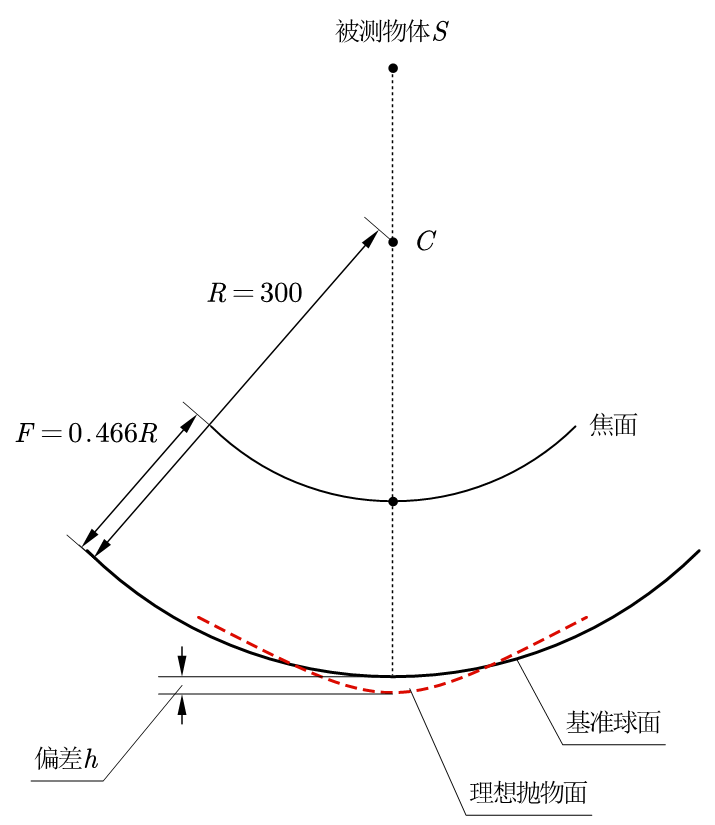
\includegraphics[height=7cm,width=7cm]{理想抛物面示意图}
				\caption{理想抛物面示意图}
				\label{理想抛物面示意图}
			\end{minipage}%
			\hfill
			\begin{minipage}[t]{0.5\linewidth}
				\centering
				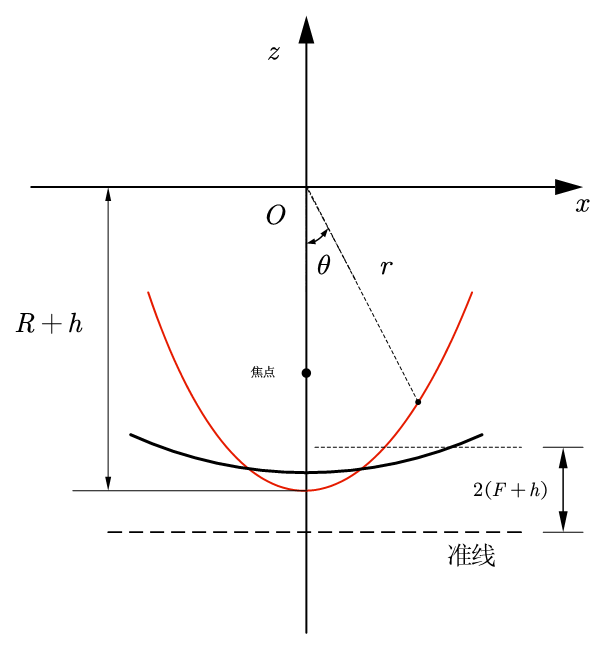
\includegraphics[height=7cm,width=8.7cm]{理想抛物面极坐标平面示意图}
				\caption{理想抛物面极坐标平面示意图}
				\label{理想抛物面极坐标平面示意图}
			\end{minipage}
		\end{figure}

		设$h$表示抛物面顶点与基准球面的垂直距离,$P$为抛物面的焦距,由$F=0.466R$,求得焦距$P=2(F+h)$。已知了焦点位置和焦距,则抛物线方程可唯一确定。$\theta$表示抛物线上各点与原点连线同$z$轴夹角,此时的抛物线方程在直角坐标系下的一般形式为:
		\begin{equation}\label{basic}
			x^2=2P(z+R+h)
		\end{equation}
		根据$x,z$和$r,\theta$的对应关系:
		\begin{equation}\label{xzr}
		\left\{ \begin{array}{c}
		x=r\sin \theta\\
		z=-r\cos \theta\\
		\end{array} \right. 
		\end{equation}
		将方程转换为极坐标系下,得到抛物面的极坐标方程:
		\begin{equation}\label{jizuobiao}
			r^2sin^2\theta=2P(-rcos\theta+R+h)
		\end{equation}
		将$r$视作因变量,$\theta$作为自变量,通过求根公式解得r与$\theta$的显式关系(另一解不满足实际情况,舍去):
		\begin{equation}\label{xianshi}
			r=\frac{-2Pcos\theta + \sqrt{4P^2cos^2\theta+4sin^2\theta\cdot 2P(R+h)}}{2sin^2\theta}
		\end{equation}
		设$M$为主索节点的集合,对于某个主索节点$M_i$,($i$为节点编号,$i=1,2,... n$,$n$为节点个数),其XYZ坐标为$(x_i,y_i,z_i)$,其到原点的距离$D_i$为
		\begin{equation}\label{key}
		D_i=\sqrt{x_i^2+y_i^2+z_i^2}
		\end{equation}
		由题可知,通过天体所在方位可以确定抛物面的旋转对称轴,设旋转对称轴的方向向量为$\vec{K}$,则由方位角 $\alpha$和仰角$\beta$确定其表达式为
		\begin{equation}\label{K}
		\vec{K}=\left( -\cos \beta \cos \alpha ,-\cos \beta \sin \alpha ,-\sin \beta \right) 
		\end{equation}
		以基准球面的球心C作为原点,则球心C的XYZ坐标为$(0,0,0)$,设某个主索节点$M_i$的XYZ坐标为$(x_i,y_i,z_i)$,向量$\vec{CM_i}$与旋转对称轴向量$\vec{K}$的夹角为$\theta_i$,由向量夹角公式可得:
		\begin{equation}\label{costheta}
		\theta_i =arccos \frac{\overrightarrow{K}\cdot \overrightarrow{CM_i}}{\left| \overrightarrow{K} \right|\,\,\left| \overrightarrow{CM_i} \right|}
		\end{equation}
		由于主索节点径向移动,因此移动前后的$\theta_i$不变,由抛物面的极坐标方程式(\ref{xianshi})求得同一夹角下抛物面上的点到原点的距离$r_i$,即:
		\begin{equation}\label{xianshi2}
		r_i=\frac{-Pcos\theta_i + \sqrt{P^2cos^2\theta_i+sin^2\theta_i\cdot 2P(R+h)}}{sin^2\theta_i}
		\end{equation}
		则主索节点$M_i$沿径向移动的距离$\Delta d_i$为:
		\begin{equation}\label{Deltad}
		\Delta d_i=r_i-D_i
		\end{equation}
		\subsubsection{问题一单目标优化模型的建立}
		\paragraph{1.优化目标}
	
		给定抛物面顶点与基准球面的垂直距离$h$的值,根据式(\ref{Deltad})可以求得每个主索节点移动到理想抛物面的位移。
		
		根据工程实际要求,结合反射面板调节的因素,主索的过度紧绷或松弛导致应力过大,对工程的寿命与精度都有一定的影响,为避免这种情况,主索节点的位移应在合理范围内且尽可能的小。各节点仅能沿径向移动,所以应使各节点到达抛物面所需的平均径向距离最小,基于此标准对决策变量$h$提出优化目标:
		\begin{equation}\label{mb1}
		\min\text{ }D=\sqrt{\frac{\sum_{i=1}^n{\Delta d_i^2}}{n}}
		\end{equation}
		其中$D$为各节点径向移动距离均方。
		\paragraph{2.约束条件}
		
		因为抛物面的口径为300m,又由于球面半径为300.4m,抛物面的左右边缘点与球心构成等边三角形,因此边缘点与原点的连线同旋转对称轴的夹角为$30^\circ$。对于需要移动的主索节点,其与原点的连线同旋转对称轴的夹角必然小于等于$30^\circ$,如图\ref{主索节点径向位移}所示。因此需要移动的主索节点满足的约束条件为:
		\begin{equation}\label{ys1}
		\theta_i \leqslant 30^\circ
		\end{equation}
		
				\begin{figure}[!htp]
			\centering
			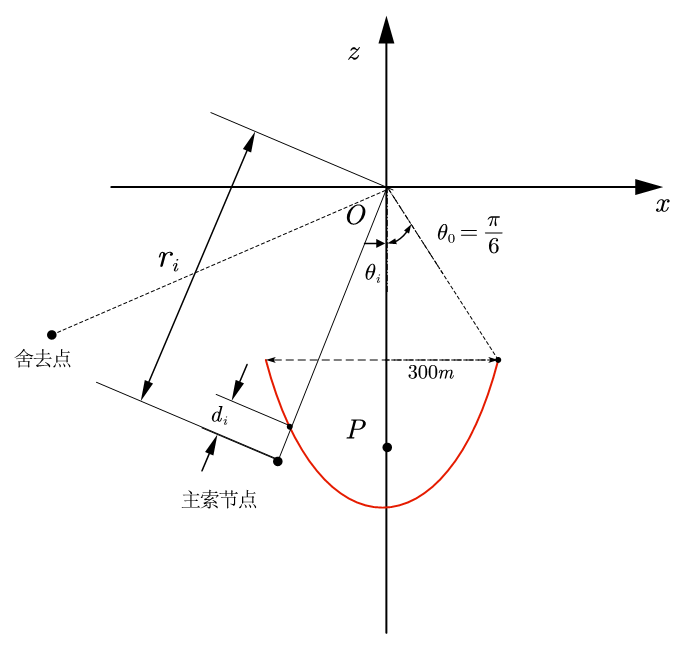
\includegraphics[width=0.6\textwidth]{主索节点径向位移}
			\caption{主索节点径向位移}
			\label{主索节点径向位移}
		\end{figure}
		
		
		综上,可以建立以$h$为决策变量,径向移动距离均方最小为目标函数的单目标规划模型:
		\begin{equation}
		\begin{aligned}
		&\hat{h}=\underset{h}{\arg } \min D=\sqrt{\frac{\sum_{i=1}^{n} \Delta d_{i}^{2}}{n}}\\
		&\left\{\begin{array}{l}
		\theta_{i}=\arccos \frac{\vec{K} \cdot \overrightarrow{C M}_{i}}{|\vec{K}| \overline{C M}_{i}} \leqslant 30^{\circ} \\
		r_{i}=\frac{-P \cos \theta_{i}+\sqrt{P^{2} \cos ^{2} \theta_{i}+\sin ^{2} \theta_{i} \cdot 2 P(R+h)}}{\sin ^{2} \theta_{i}} \\
		D_{i}=\sqrt{x_{i}^{2}+y_{i}^{2}+z_{i}^{2}} \\
		\Delta d_{i}=r_{i}-D_{i}
		\end{array}\right.
		\end{aligned}
		\end{equation}
		
		
		
		
		\subsubsection{基于黄金分割法优化求解h}
		根据附件一中主索节点的坐标,计算各节点在极坐标系下的$r_i$与$\theta_i$,判断是否满足$\theta_i\le\frac{\pi}{6}$,满足条件的节点即为需要移动以拟合理想抛物面的节点,反之舍去。
		
		
		在问题1中,$\alpha=0^\circ,\beta=90^\circ$,以$0m$为初值,$0.01m$为步长,$0.6m$为终值遍历$h$,求出相应的径向移动距离均方$D$,得到的关系图如图\ref{问题1径向移动均方距离随h的变化}。
			\begin{figure}[!htp]
			\centering
			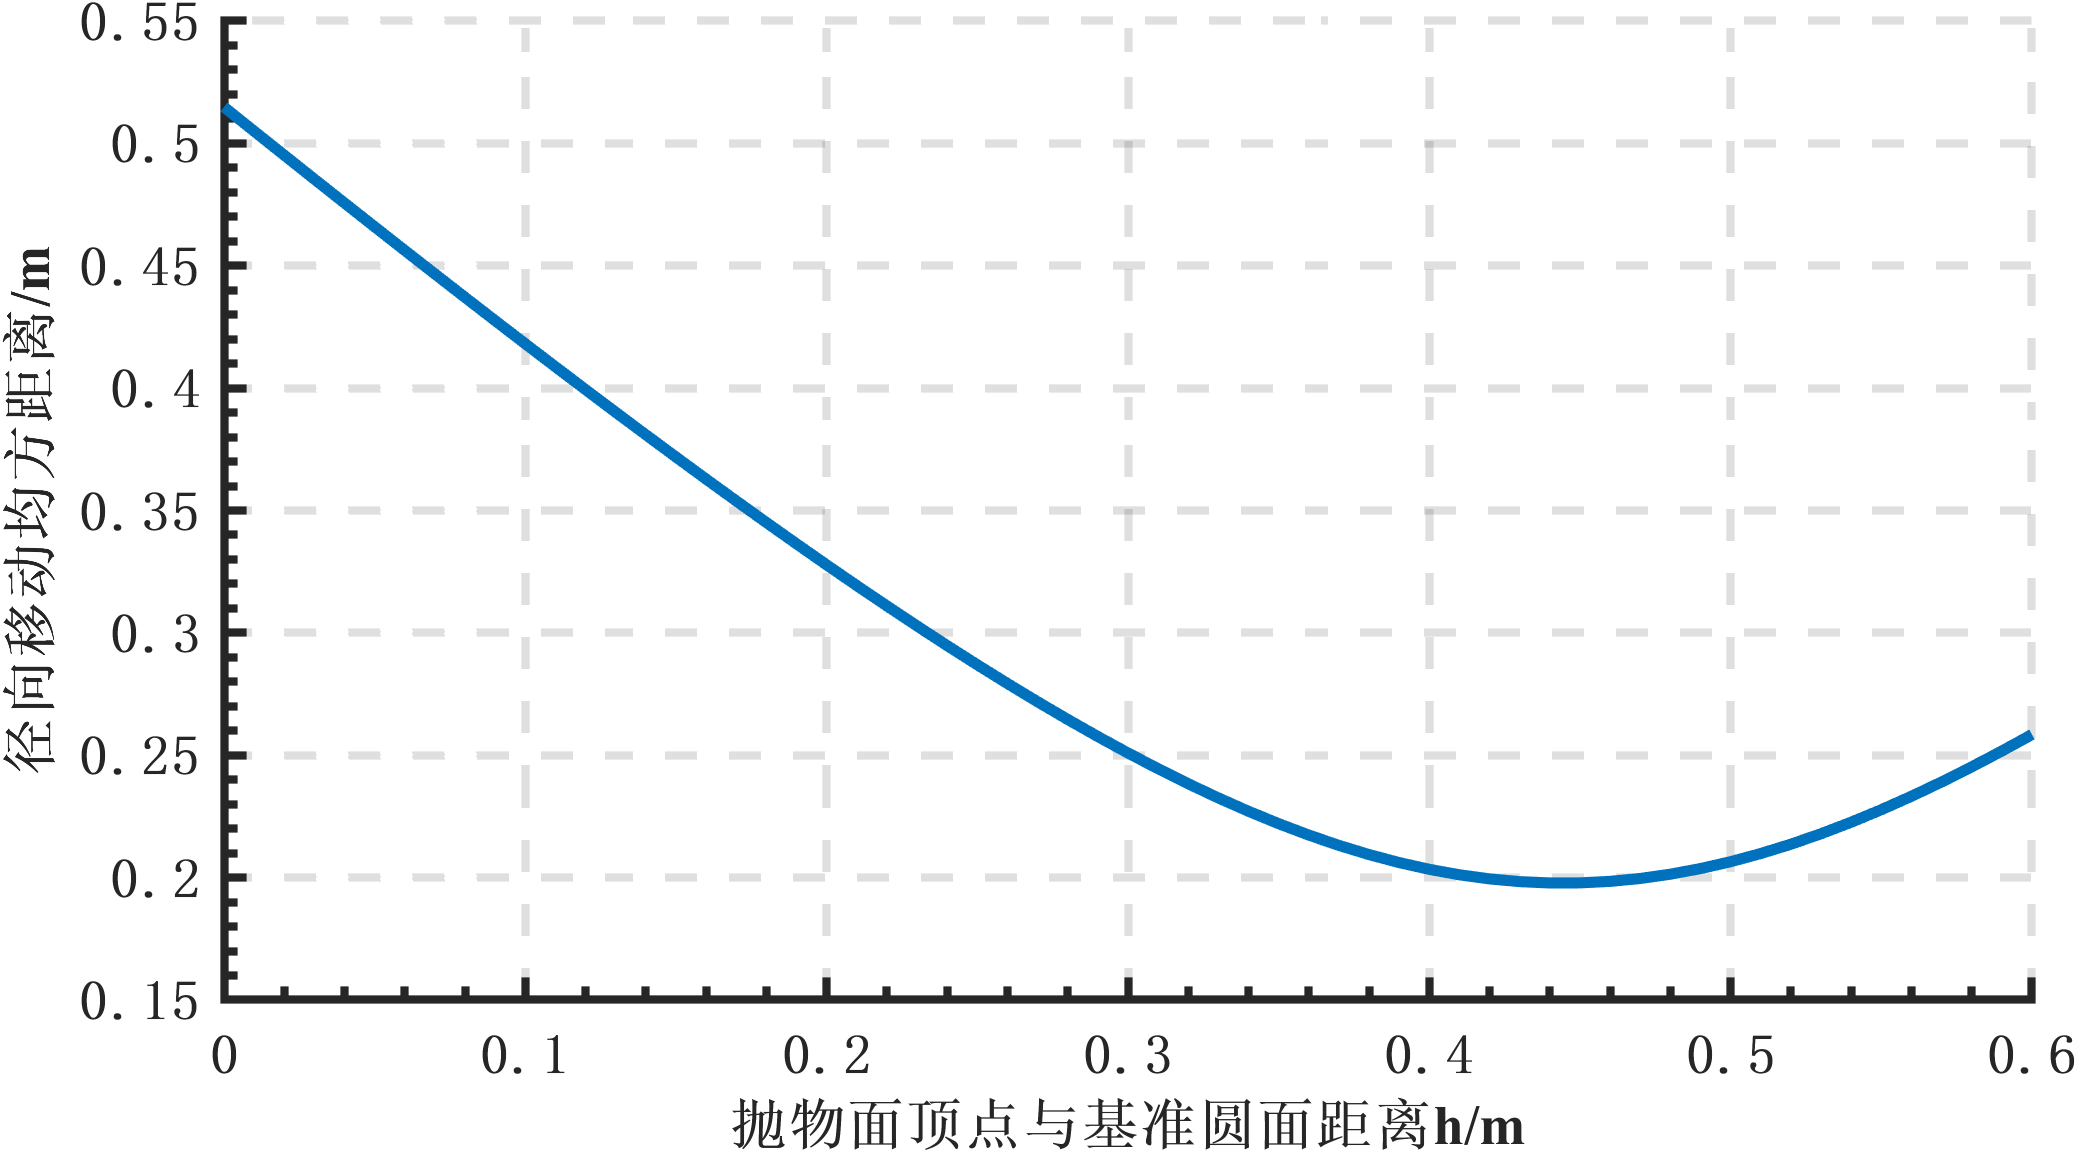
\includegraphics[width=0.75\textwidth]{问题1径向移动均方距离随h的变化}
			\caption{问题1径向移动均方距离随h的变化}
			\label{问题1径向移动均方距离随h的变化}
		\end{figure}
		
		根据曲线图,初步判断$D$随$h$增长的关系$D$是先减后增,则问题转换为求$D$在区间$[0m,0.6m]$的极小值点$h^{*}$。 $D$关于h的函数为区间$[0m,0.6m]$上的下单峰函数,可采用采用一维搜索方法的黄金分割法进行求解。求解步骤如下:
		
		 \textbf{STEP1:}在初始区间[a,b]长度的0.618处和0.382处分别插入两点$h_1,h_2$,称作搜索点,计算并比较$D(h_1),D(h_2)$。
		 
		 \textbf{STEP2:}对于单下峰函数,当$D(h_1)<D(h_2)$时,必有$h^*\in[h_1,b]$;当$D(h_1)>D(h_2)$时,则有$h^*\in[a,h_2]$。据此更新区间。
		 
		 \textbf{STEP3:}更新区间,当区间长度小于精度$\delta$时(取0.0001),选取此区间内的任一搜索点作为$h^*$的近似解。否则,再次插入新的搜索点,进行迭代运算。
		
	
		根据算法,编程最终求得$h=0.4444m$。据此,即可确定理想抛物面。
		
	
	
	\subsection{问题二模型的建立和求解}
	\subsubsection{问题二理想抛物面的确定}
		问题二中的被测物体的位置有了方向的变换,利用问题一建立的模型,调整方位角$\alpha= 36.795°$, 仰角$\beta = 78.169°$,求得旋转对称轴的方向向量为
		\begin{equation}\label{K2}
		\vec{K}=\left( -\cos \beta \cos \alpha ,-\cos \beta \sin \alpha ,-\sin \beta \right) =(-0.1642,-0.12282,-0.9788)
		\end{equation}
		利用问题1的算法,计算得到此时的偏移量$h=0.4380m$,据此确定此时的理想抛物面。则抛物面的顶点坐标为
		\begin{equation}\label{ddzb}
		(R+h)\vec{K}=(-49.3919,-36.9432,-294.4472)
		\end{equation}
	
	\subsubsection{问题二各主索点径向位移的求解}
		问题需要使工作平面尽可能地贴近理想抛物面,该拟合过程可看作参数优化过程,其优化参数为主索节点与抛物面之间的径向距离。将三个相互连接的主索节点构成的三角形反射单元看作平面,从抛物面的侧面看去,由图\ref{问题2最优主索节点位置的比较}所示。
			\begin{figure}[!htp]
			\centering
			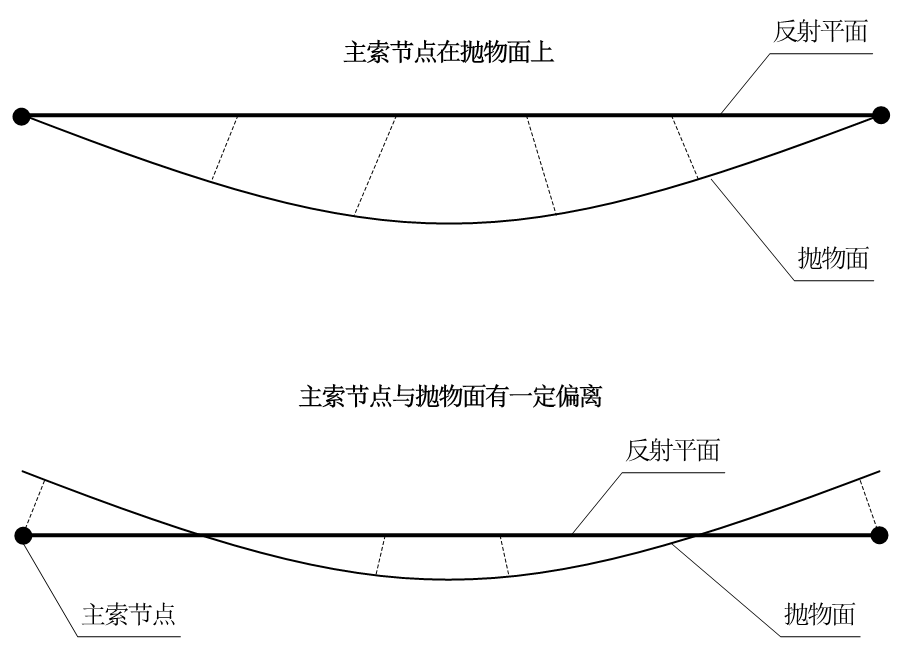
\includegraphics[width=0.6\textwidth]{问题2最优主索节点位置的比较}
			\caption{问题2最优主索节点位置的比较}
			\label{问题2最优主索节点位置的比较}
		\end{figure}
		显然并非当主索节点落在抛物面上时,拟合精度最好,而是当又有一定偏离,使反射平面与抛物面的整体距离最小,达到最优拟合精度。
		
		各主索点径向位移的求解步骤如下:
		
		\textbf{步骤一:确定初始位移}
		
		计算各主索节点到理想抛物面的径向距离$\Delta D0$,将主索节点径向移动到抛物面上,即第一步的位移为$\Delta D0$。此时得到一个较好的初始解,但此时的解并不是最优;
		
		\textbf{步骤二:计算每个主索节点周围统计点到抛物面平均距离和误差}
		
		为得更优的位移量,首先确定各主索节点连接的反射平面,借助数值积分的思想,在每个主索节点周围的若干三角形平面单元上均匀地选取若干个统计点,如图\ref{问题2周围统计点}所示。计算周围各统计点与理想抛物面的平均径向距离$\Delta D1$(有正有负),并计算各统计点与理想抛物面的径向距离的均方根值$RMS$(即公式(\ref{mb1}))
		
		\begin{equation}\label{}
		RMS=\sqrt{\frac{\sum_{i=1}^n{\Delta d_i^2}}{n}}
		\end{equation}
		对每个主索节点的RMS求和取平均再开平方,得到总的误差RMS。
			\begin{figure}[!htp]
			\centering
			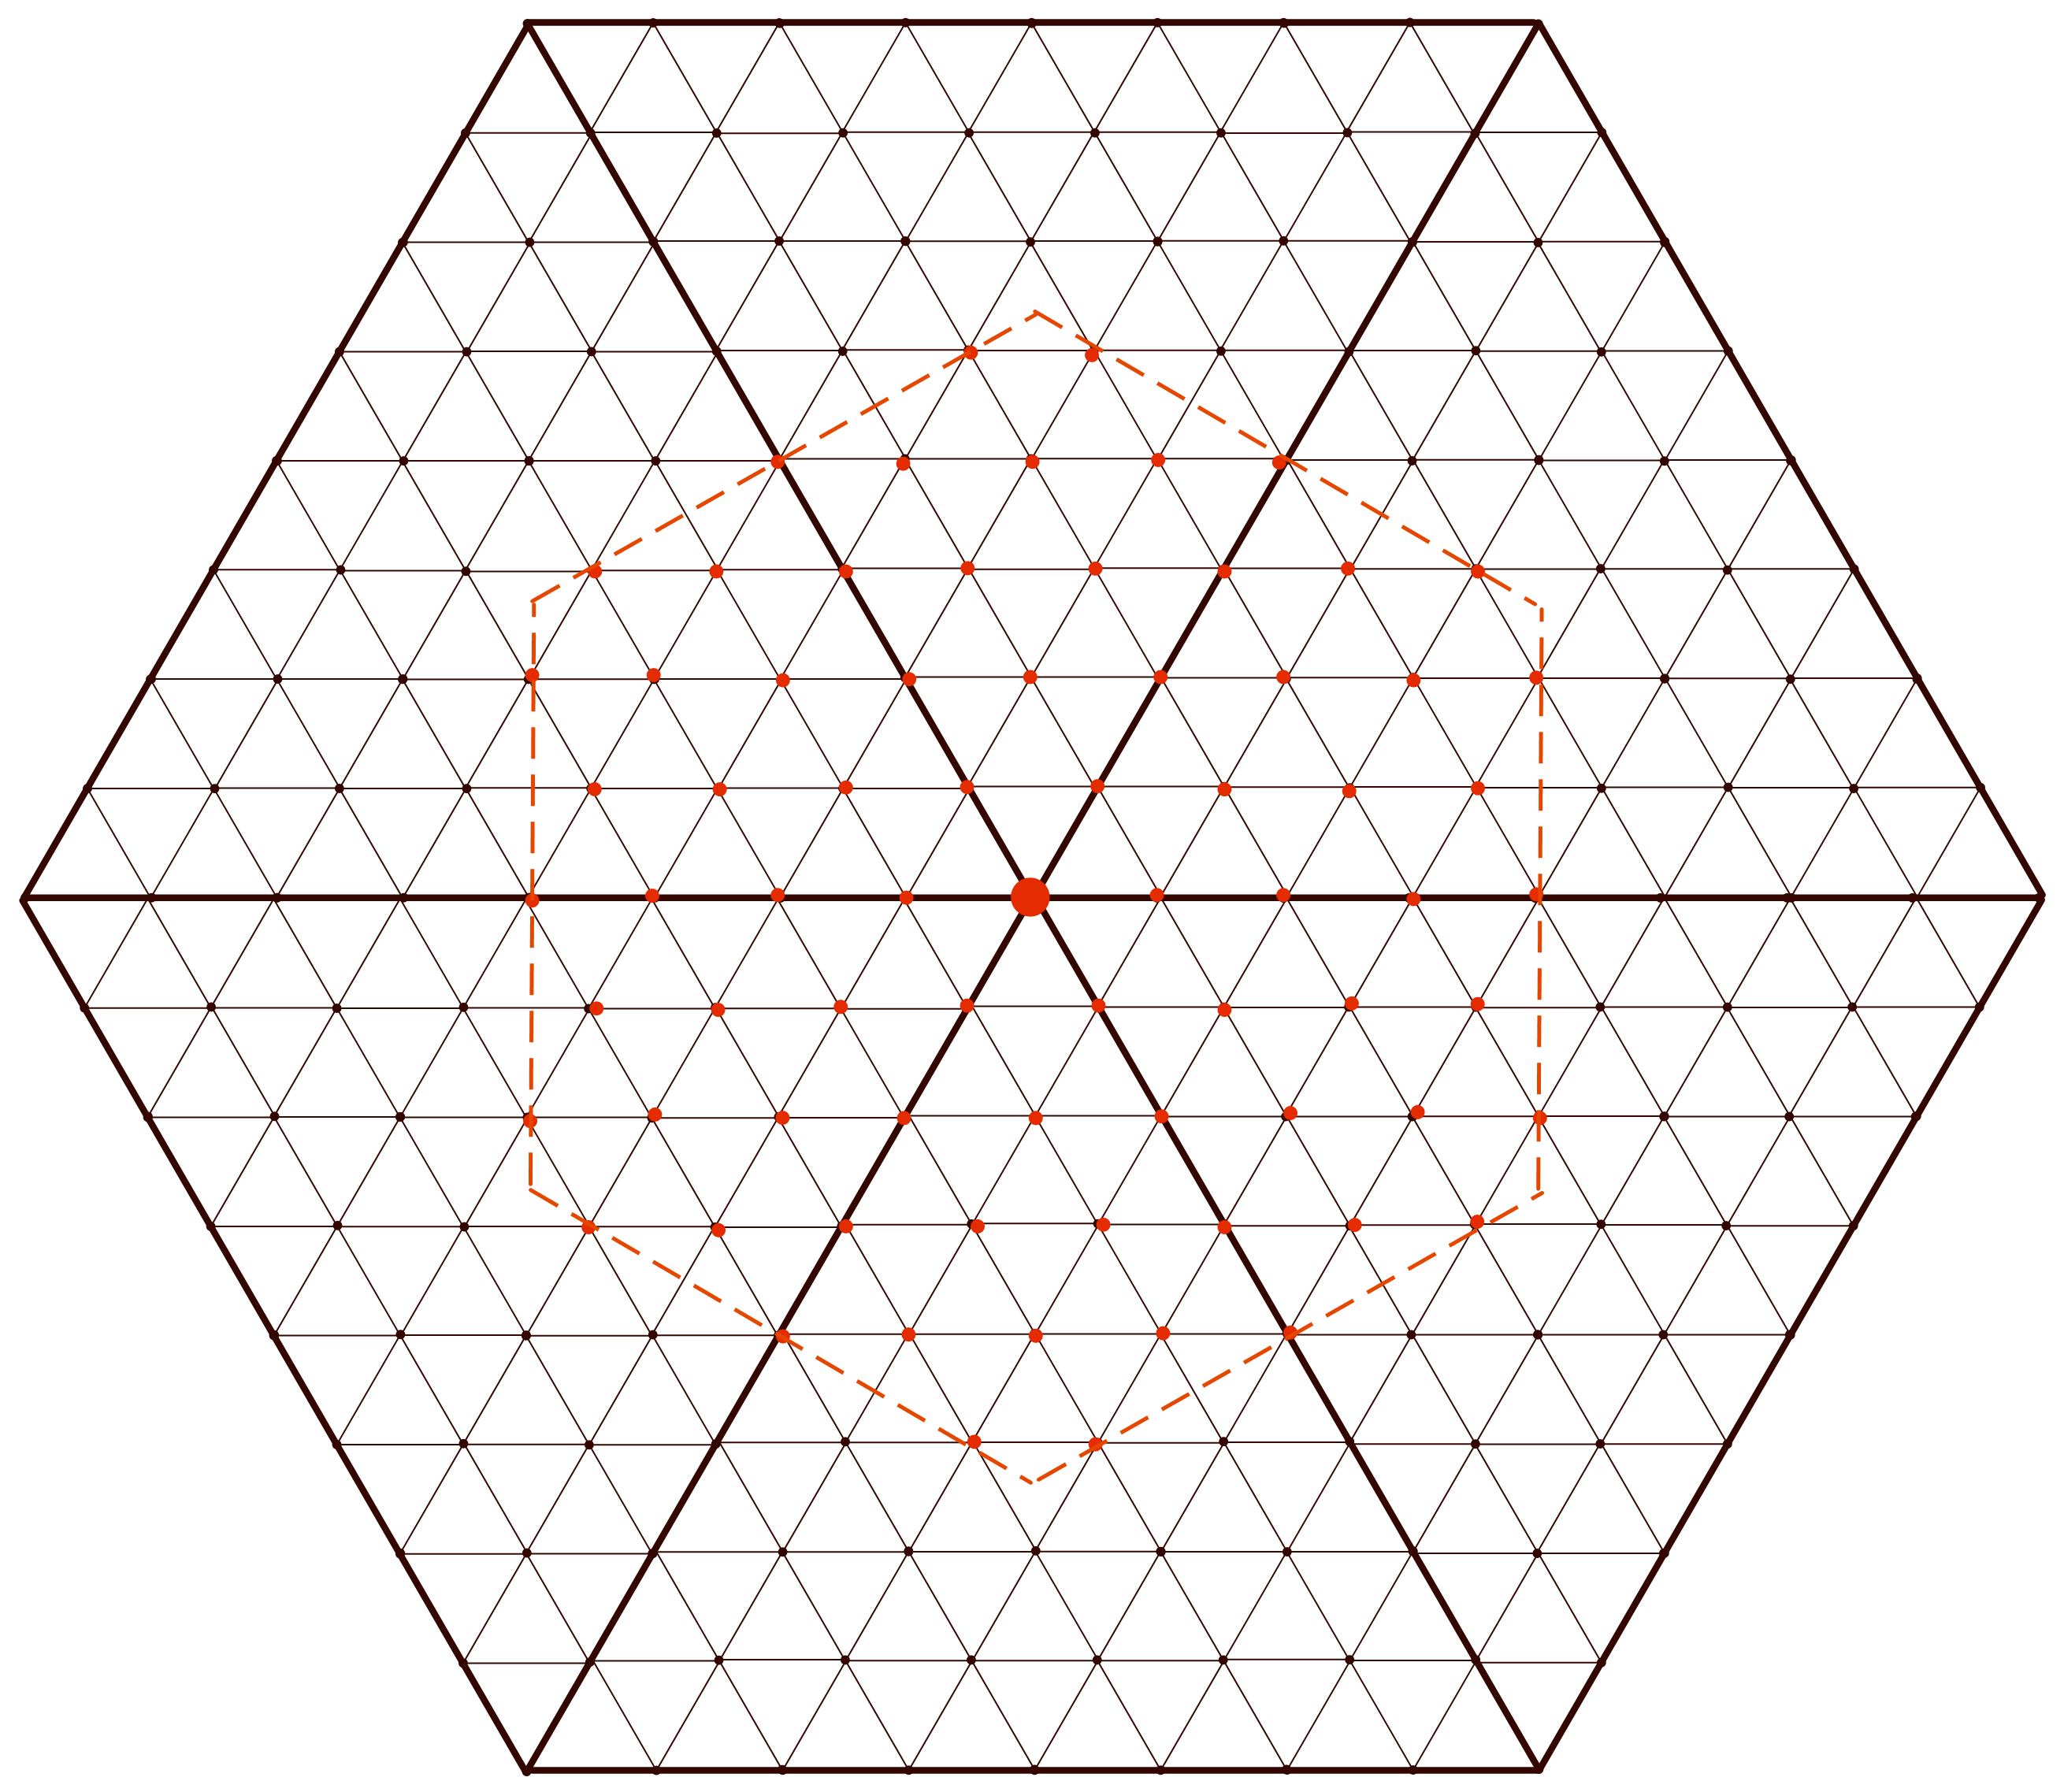
\includegraphics[width=0.6\textwidth]{问题2周围统计点}
			\caption{问题2周围统计点}
			\label{问题2周围统计点}
		\end{figure}
		为了得到$\Delta D1$和$RMS$,需要遍历该主索节点周围的三角形平面,得到所有统计点的XYZ坐标。以单个三角形平面为例,如图\ref{问题2单个三角形平面统计点}所示。
		
			\begin{figure}[!htp]
			\centering
			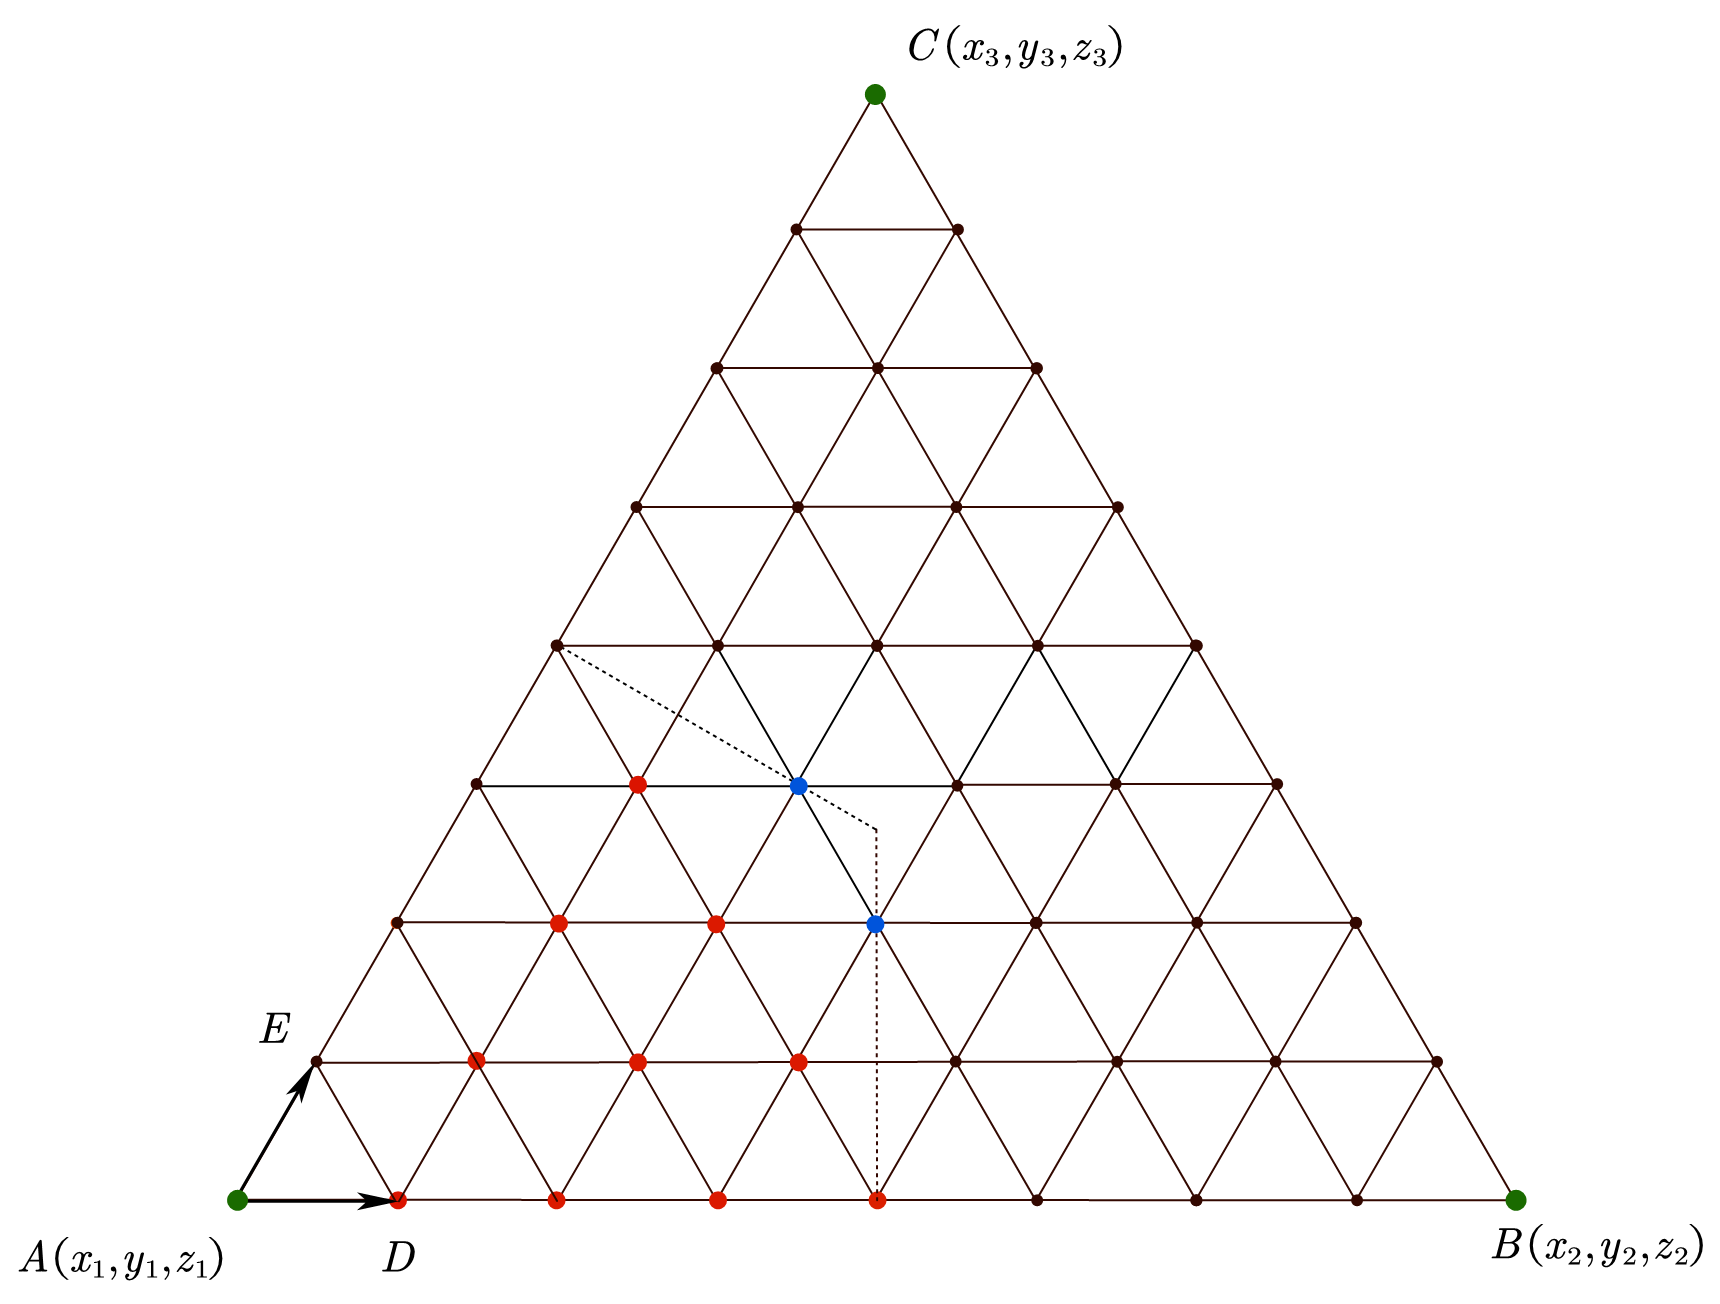
\includegraphics[width=0.6\textwidth]{问题2单个三角形平面统计点}
			\caption{问题2单个三角形平面统计点}
			\label{问题2单个三角形平面统计点}
		\end{figure}
		在图\ref{问题2单个三角形平面统计点}中,A点为我们讨论的主索节点,A与B、C两个节点构成三角形平面。将三角形的3条边8等分,对于图\ref{问题2单个三角形平面统计点}中红色标注的统计点,其XYZ坐标的递推公式为
	\begin{equation}
	\begin{gathered}
	P(x, y, z)=A(x, y, z)+i \cdot \overrightarrow{A D}+j \cdot \overrightarrow{D E} \\
	i=1,2,3,4 ; j=0, \ldots, i-1 \\
	\overrightarrow{A D}=\overrightarrow{A B} / 8 ; \overrightarrow{A E}=\overrightarrow{A C} / 8 \\
	D(x, y, z)=A(x, y, z)+\overrightarrow{A D} \\
	E(x, y, z)=A(x, y, z)+\overrightarrow{A E} \\
	\overrightarrow{D E}=E(x, y, z)-D(x, y, z)
	\end{gathered}
	\end{equation}
	
	对于外围2个蓝色的点,其递推公式为:
	\begin{equation}
	P(x, y, z)=A(x, y, z)+5 \cdot \overrightarrow{A D}+\left\{\begin{array}{l}
	2 \overrightarrow{D E} \\
	3 \overrightarrow{D E}
	\end{array}\right.
	\end{equation}
		
		\textbf{步骤三:以步骤二中得到的平均距离反向移动各主索节点}
		
		在步骤二中得到了各主索节点周围统计点平均距离$\Delta D1$,反向移动各主索节点,重新计算总和RMS。重复步骤二,进行迭代计算,直到$RMS$值趋于稳定,本模型中的判断标准选取的是前后的RMS差值小于0.001。
		
		最终总和的径向位移为$\Delta D=\Delta D0+\Delta D1+...$,移动后主索节点的XYZ坐标由原来的位置坐标径向移动$\Delta D$后得到。
	
	\subsubsection{问题二径向位移和坐标求解结果}

	\textbf{1.主索节点位移与促进器伸缩量的讨论}
	
	现讨论主索节点伸缩量与对应促进器伸缩量的关系。节点、促进器顶端与基准球面球心三点并不在同一直线上,节点与促进器均沿径向移动,且连接两者的下拉索长度固定,如图\ref{主索节点偏移}显示
	\begin{figure}[H]
		\centering
		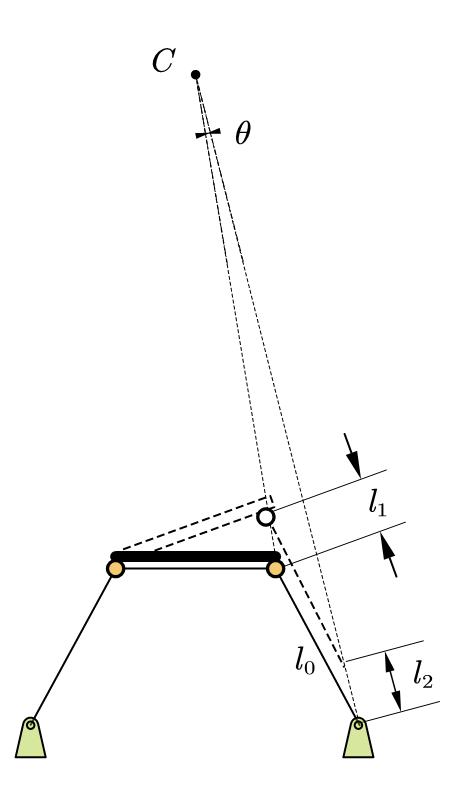
\includegraphics[height=0.6\textwidth]{主索节点偏移.png}
		\caption{主索节点偏移}\label{主索节点偏移}
	\end{figure}
	
	设节点坐标$(r_1,\theta_1)$,促进器上端坐标$(r_2,\theta_2)$,节点和促进器上端的径向移动距离分别是$l_1,l_2$,则由余弦定理可以得到关系式:
	\begin{equation}\label{节点偏移余弦}
	cos\theta = \frac{(r_1-l_1)^2+(r_2-l_2)^2-l_0^2}{2(r_1-l_1)(r_2-l_2)}
	\end{equation}
	
	$l_0$是拉索长度,为已知量,则得到了$l_1$与$l_2$的关系式,可由主索节点的偏移计算出对应促进器的伸缩量。
	
	将附件1附件2中各点坐标值导入计算夹角余弦值$cos\theta$,得到的结果均接近于1,精度达到了0.0000001,则可以认为基准球面球心、主索节点和促进器顶端在同一直线上,在模型建立与计算过程中可视作$l_1=l_2$,即主索节点的偏移等于促进器的伸缩量。
	
	\textbf{2.促进器伸缩量和调整后主索节点坐标求解结果}
	
		由上述迭代方法,计算位移量和位移后坐标,前10个主索节点的编号、移动后XYZ坐标和促进器伸缩量如表\ref{前10个主索节点的编号、移动后XYZ坐标和促动器伸缩量}。误差RSM收敛过程如图\ref{均方误差RSM随迭代次数的变化},由图可知,迭代两次即收敛。
		\begin{figure}[!htp]
			\centering
			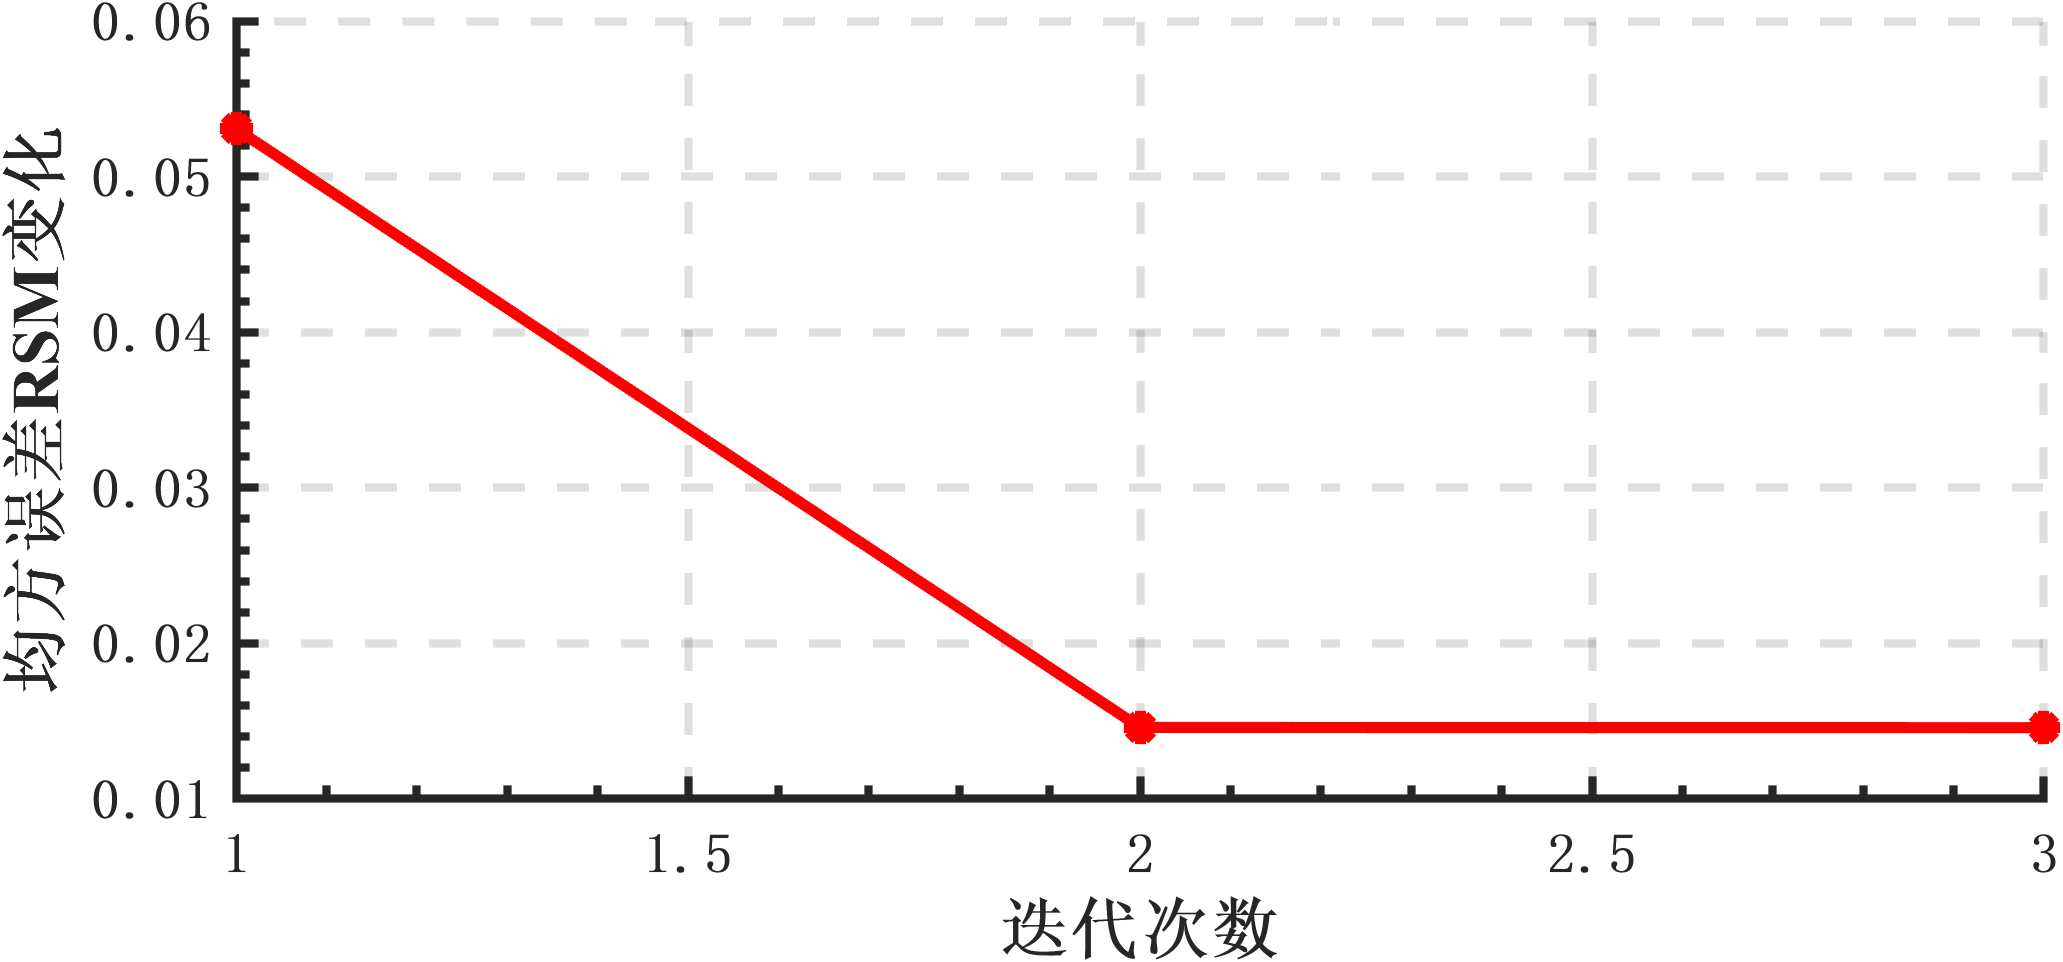
\includegraphics[width=0.6\textwidth]{均方误差RSM随迭代次数的变化}
			\caption{均方误差RSM随迭代次数的变化}
			\label{均方误差RSM随迭代次数的变化}
		\end{figure}
		
	% Table generated by Excel2LaTeX from sheet 'Sheet1'
	\begin{table}[htbp]
		\centering
		\caption{前10个主索节点的编号、移动后XYZ坐标和促动器伸缩量}
		\begin{tabularx}{\textwidth}{@{}c *4{>{\centering\arraybackslash}X}@{}}
			\toprule[1.5pt]
			节点编号  & X坐标(米) & Y坐标(米) & Z坐标(米) & 伸缩量(米) \\
			\midrule
			A0    & 0     & 0     & -300.5107 & -0.1107 \\
			B1    & 6.108298 & 8.407685 & -300.2447 & -0.024492 \\
			C1    & 9.884553 & -3.211602 & -300.2765 & -0.056327 \\
			D1    & 0     & -10.39692 & -300.3913 & -0.17119 \\
			E1    & -9.889597 & -3.213241 & -300.4297 & -0.20966 \\
			A1    & -6.11 & 8.410028 & -300.3283 & -0.10821 \\
			A3    & 0     & 16.81867 & -299.9409 & -0.012042 \\
			B2    & 12.20589 & 16.80055 & -299.6195 & 0.061749 \\
			B3    & 15.99264 & 5.196494 & -299.8997 & 0.029247 \\
			C2    & 19.75289 & -6.41777 & -299.6704 & 0.010753 \\
			\bottomrule[1.5pt]
		\end{tabularx}%
		\label{前10个主索节点的编号、移动后XYZ坐标和促动器伸缩量}%
	\end{table}%
	
	由于径向伸缩范围为 -0.6到0.6 米,因此检查求解结果的最大位移量为$0.4977m$,满足要求,因此此时求得的结果为最优结果。移动前后主索节点的位置分布如图\ref{问题2原始节点和调整后节点}。
	\begin{figure}[!htp]
		\centering
		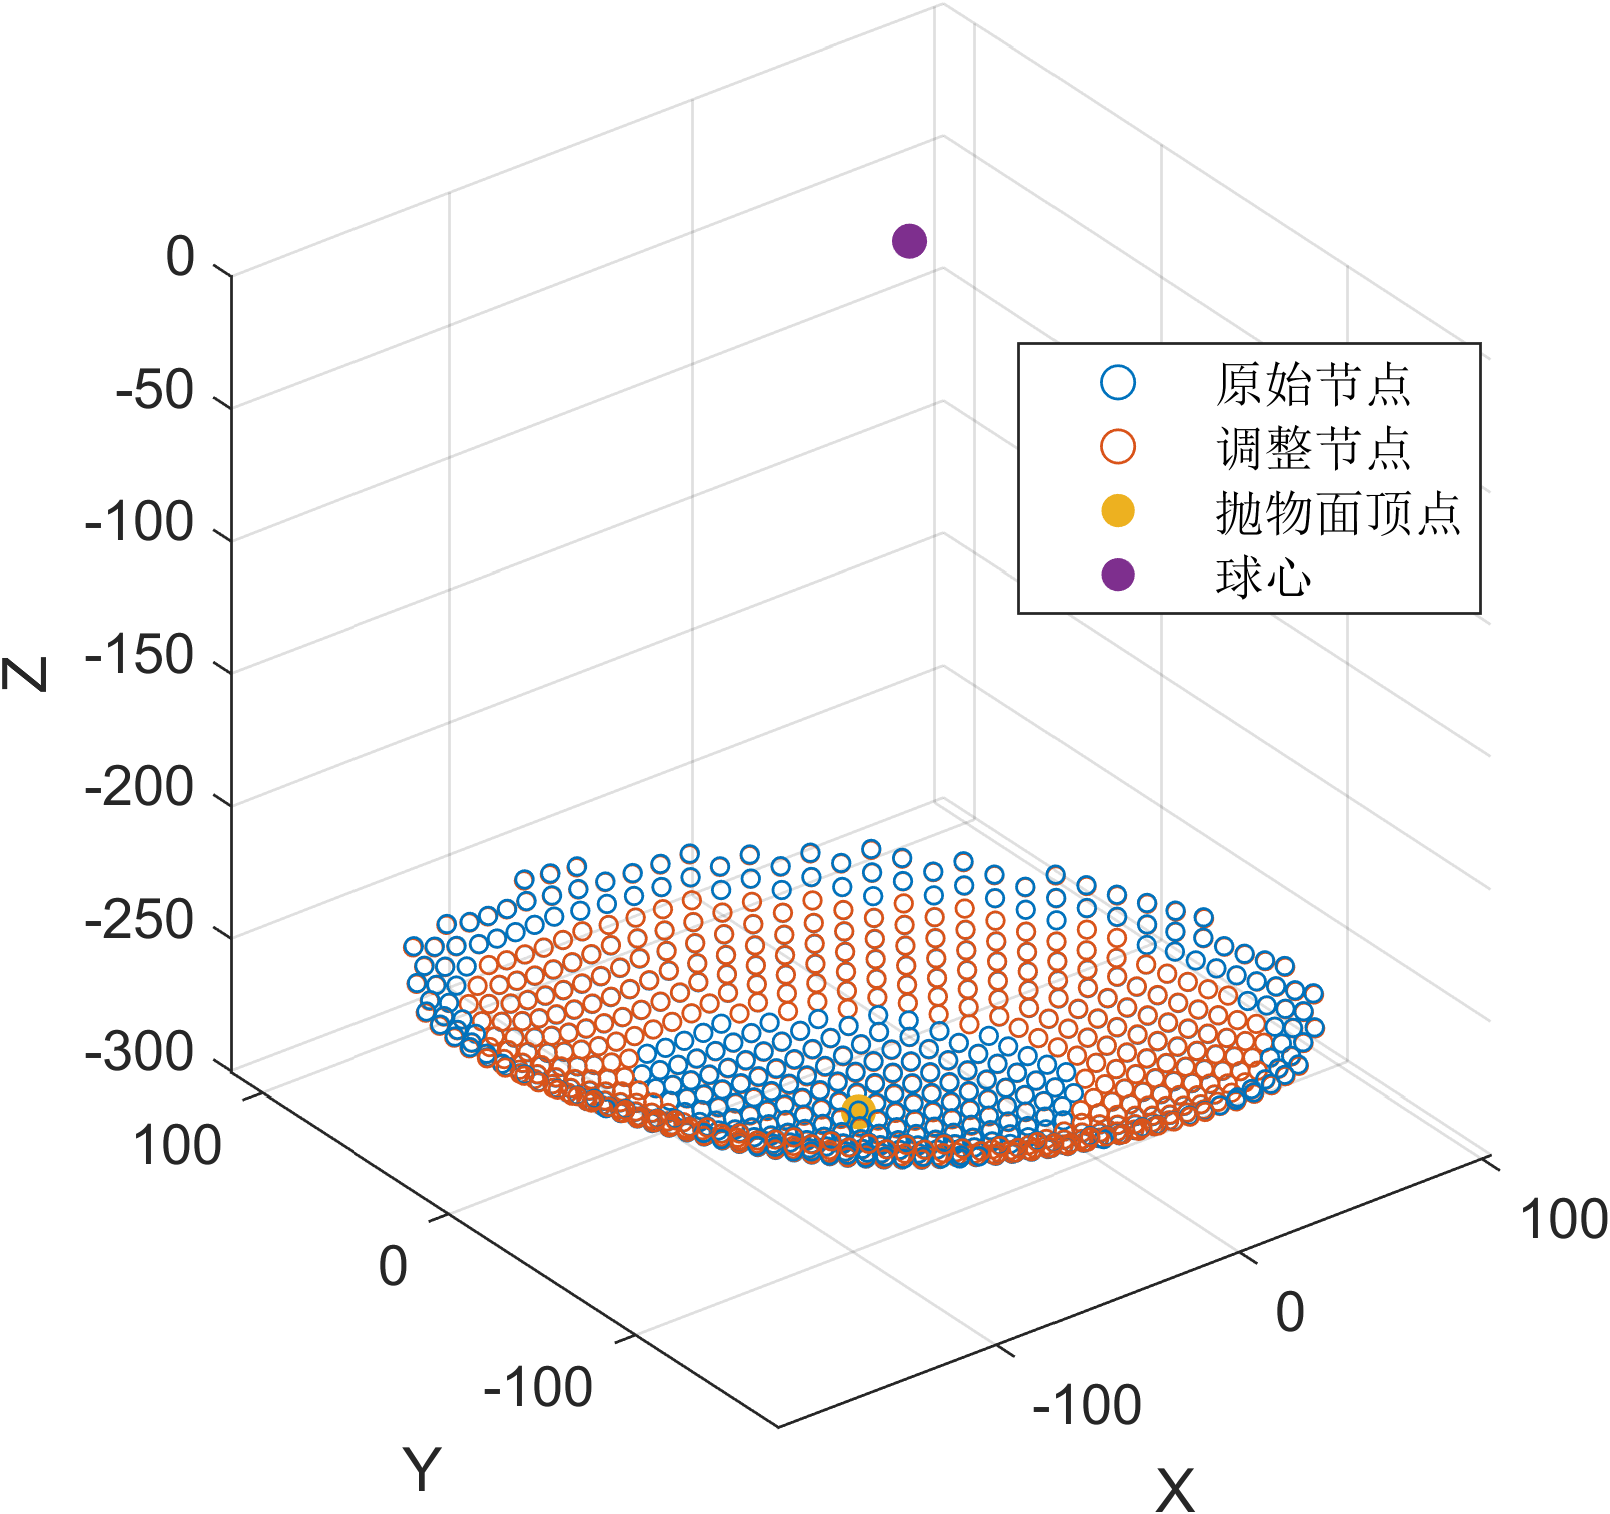
\includegraphics[width=0.6\textwidth]{问题2原始节点和调整后节点}
		\caption{问题2原始节点和调整后节点位置分布}
		\label{问题2原始节点和调整后节点}
	\end{figure}
	
	\subsection{问题三模型的建立和求解}
	\subsubsection{坐标系旋转} 
	问题二中求得的抛物面开口指向被测天体,在原始坐标系下呈斜向状态,中轴与z轴之间有较大的夹角,使得对应的抛物面方程较为复杂,计算困难,不便于光线反射的求解,通过对坐标系的旋转操作,将旋转后的z轴与基准球面球心同被测天体的连线重合,此时的抛物面转换为了问题一中的状态,电磁波沿z轴负方向竖直射下,大大简化了计算。
	\begin{figure}[H]
		\centering
		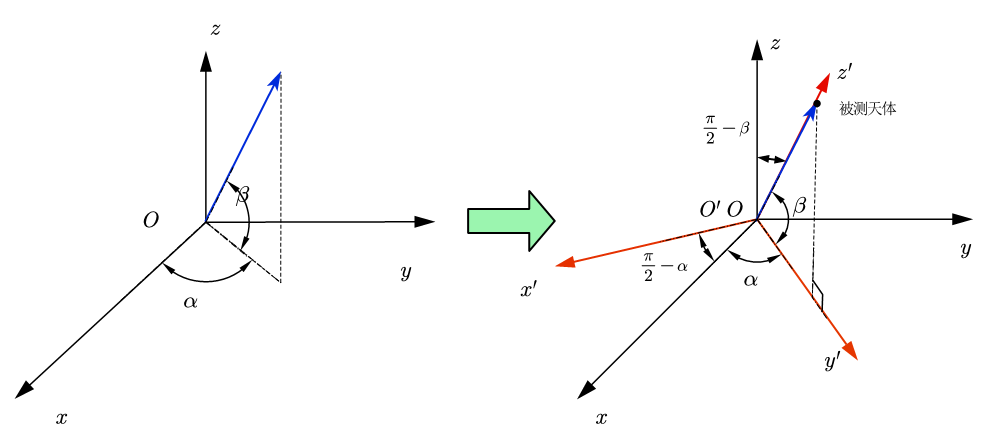
\includegraphics[width=0.8\textwidth]{坐标系旋转示意.png}
		\caption{坐标系旋转示意}\label{坐标系旋转示意}
	\end{figure}
	
	由图\ref{坐标系旋转示意}显示,将坐标系先绕z轴顺时针旋转$\frac{\pi}{2}-\alpha$,再绕x轴顺时针旋转$\frac{\pi}{2}-\beta$,使z轴与目标直线重合,达到目标坐标系。
	
	%\paragraph{旋转原理}
	以z轴旋转为例,考虑到旋转过程中,点在z轴上的坐标不会发生变化,为简化问题,将坐标系投影在$xOy$平面上进行求解。如图\ref{坐标系旋转平面示意}所示,其中$xOy$为原始坐标系,$x'O'y'$为旋转后的坐标系。
	
	\begin{figure}[H]
		\centering
		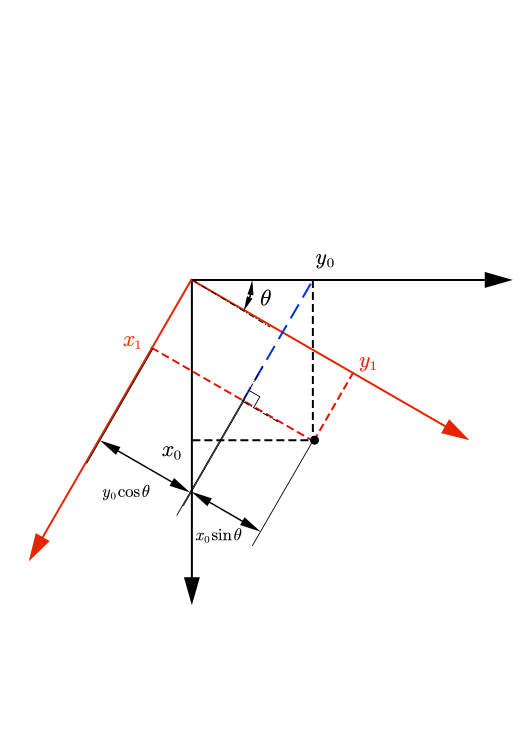
\includegraphics[height=0.6\textwidth]{坐标系旋转平面示意.png}
		\caption{坐标系旋转平面示意}\label{坐标系旋转平面示意}
	\end{figure}
	
	利用几何关系,可以求得旋转后的坐标变换公式(即求坐标轴上的投影长度):
	\begin{equation}\label{z轴旋转公式}
	\left\{ \begin{array}{l}
	x_1=x_0\cos \theta -y_0\sin \theta\\
	y_1=y_0\cos \theta +x_0\sin \theta\\
	z_1=z_0\\
	\end{array} \right. 
	\end{equation}
	
	同理,针对绕x轴的旋转坐标变换公式如下:
	\begin{equation}\label{x轴旋转公式}
	\left\{ \begin{array}{l}
	x_1=x_0\cos \theta +z_0\sin \theta\\
	y_1=y_0\\
	z_1=z_0\cos \theta -x_0\sin \theta\\
	\end{array} \right. 
	\end{equation}
	
	%\paragraph{旋转矩阵}
	借助矩阵计算,可以更快的求解旋转坐标的变换,其中$z$轴旋转矩阵:
	\begin{equation}\label{z轴旋转矩阵}
	\left[ \begin{matrix}
	\cos  \theta &		-\sin  \theta &		0\\
	\sin  \theta &		\cos  \theta &		0\\
	0&		0&		1\\
	\end{matrix} \right] 
	\end{equation}
	
	$x$轴旋转矩阵:
	\begin{equation}\label{x轴旋转矩阵}
	\left[ \begin{matrix}
	1&		0&		0\\
	0&		\cos \beta &		-\sin  \beta \\
	0&		\sin \beta &		\cos  \beta \\
	\end{matrix} \right] 
	\end{equation}
	
	
	结合被测天体的方位角和仰角,根据图\ref{坐标系旋转示意},可以确定矩阵形式的坐标变换公式:
	\begin{equation}\label{坐标变换矩阵}
	\left[ \begin{array}{c}
	x'\\
	y'\\
	z'\\
	\end{array} \right] =\left[ \begin{matrix}
	1&		0&		0\\
	0&		\cos \left( \frac{\pi}{2}-\beta \right)&		-\sin \left( \frac{\pi}{2}-\beta \right)\\
	0&		\sin \left( \frac{\pi}{2}-\beta \right)&		\cos \left( \frac{\pi}{2}-\beta \right)\\
	\end{matrix} \right] \left[ \begin{matrix}
	\cos \left( \frac{\pi}{2}-\theta \right)&		-\sin \left( \frac{\pi}{2}-\theta \right)&		0\\
	\sin \left( \frac{\pi}{2}-\theta \right)&		\cos \left( \frac{\pi}{2}-\theta \right)&		0\\
	0&		0&		1\\
	\end{matrix} \right] \left[ \begin{array}{c}
	x_0\\
	y_0\\
	z_0\\
	\end{array} \right] 
	\end{equation}
	
	其中$
	\left[ \begin{matrix}
	x_0&		y_0&		z_0\\
	\end{matrix} \right] ^T
	$表示原始坐标系下点的坐标,$
	\left[ \begin{matrix}
	x'&		y'&		z'\\
	\end{matrix} \right] ^T
	$ 表示旋转后坐标系中的坐标。
	
	\subsubsection{截面降维计算}
	问题二中求解的结果得到调整后各节点的位置坐标,由于拟合优化操作,这些节点近似分布在一个抛物面上,但仍不够精确,存在着偏差,对结果点集进行三维散点插值,得到新的更加密集的三维点,更新后的点集分布更有规律,形成的抛物面更加光滑。
	
	将插值后的各点坐标左乘旋转矩阵,得到旋转后的坐标点,此时各点拟合形成的抛物面中轴接近z轴,开口向上,电磁波竖直向下射入。整体图形具有对称性,类比问题一,可将其投影在平面上简化求解,同时根据光的反射定理,入射光、反射光与法线在同一平面上,平面的截取不会对问题求解造成影响。此处选取$xOz$平面$yOz$两个平面进行截取,得到分布在$xOz$平面$yOz$平面上的若干散点,且散点分布近似抛物线。$xOz$截面上的抛物线散点及局部放大如图\ref{问题3 ZX平面上的抛物线及局部放大}.
			\begin{figure}[!htp]
		\centering
		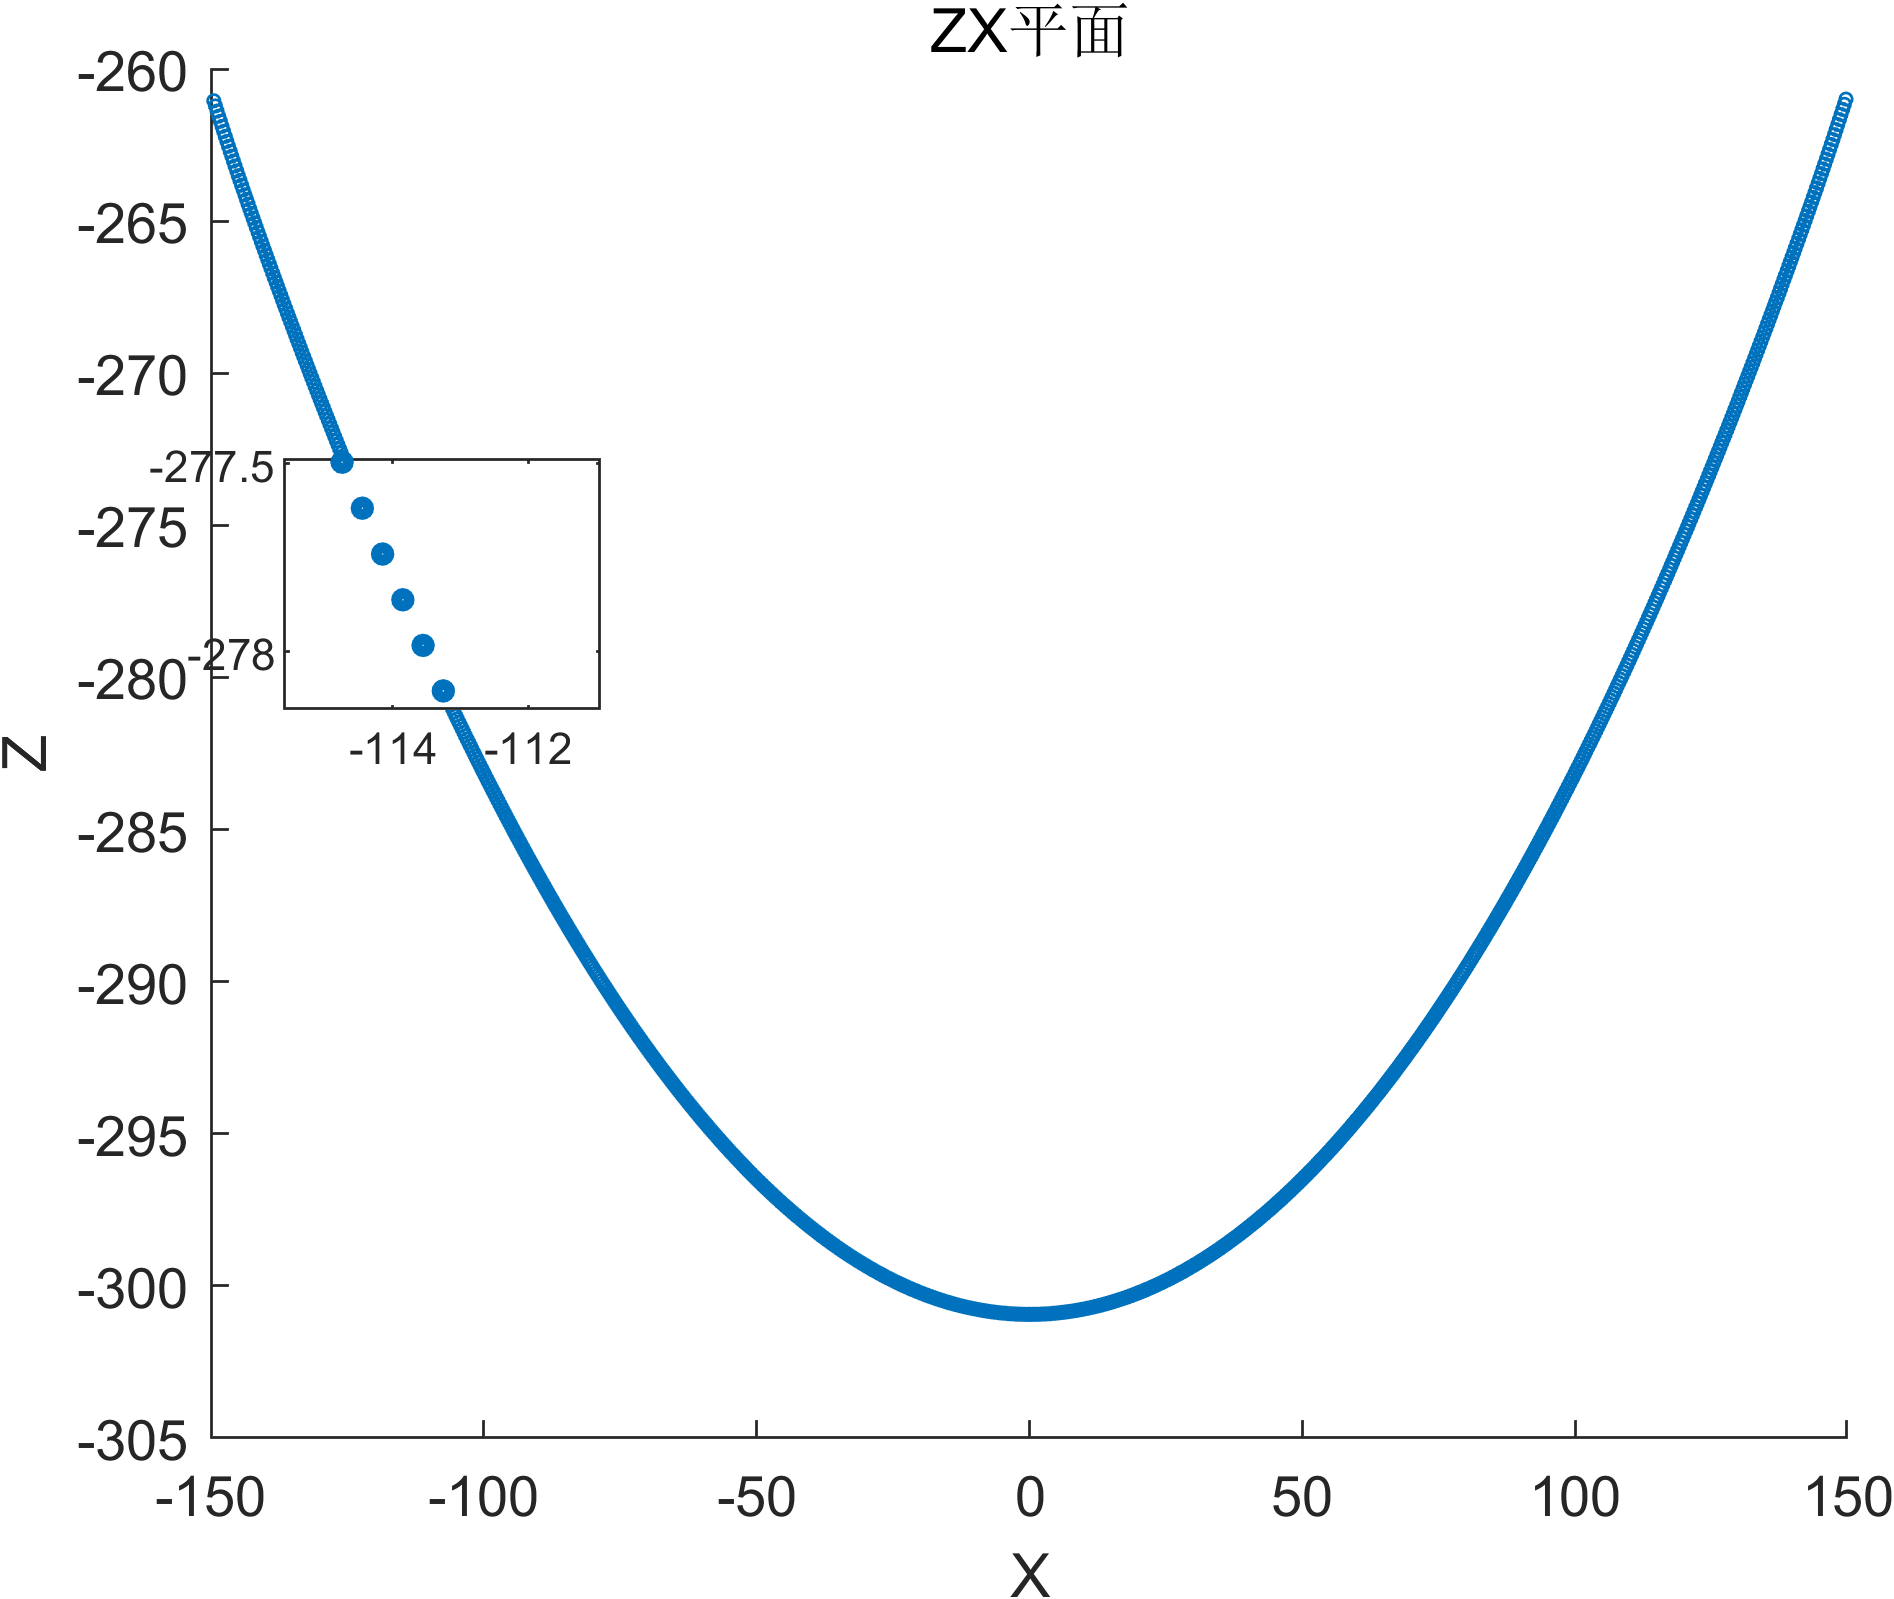
\includegraphics[width=0.6\textwidth]{问题3 ZX平面上的抛物线及局部放大}
		\caption{ZX平面上的抛物线及局部放大}
		\label{问题3 ZX平面上的抛物线及局部放大}
	\end{figure}
	图\ref{问题3 ZX平面上的抛物线及局部放大}中各散点的横轴间距是相等(插值的时候使用等间隔插值),电磁波竖直入射到这些散点上,计算反射电磁波是否反射到了馈源舱,统计反射到馈源舱的电磁波比例。
	
	因为各散点的横轴间距是相等,因此此时计算的比例即可代表$xOz$截面的接收比例。假设得到的比例为$\lambda_1$,即为$xOz$截面的接收比例。按同样的步骤计算$yOz$截面的接收比例$\lambda_2$。由于电磁波在一个面上入射,因此总的接收比例$\lambda$为:
	\begin{equation}\label{lb}
	\lambda =\left( \frac{\lambda _1+\lambda _2}{2} \right) ^2
	\end{equation}
	
	\subsubsection{截面接收比例的计算}
	以xOz截面为例,如图\ref{问题3离散抛物面反射}所示,
				\begin{figure}[!htp]
		\centering
		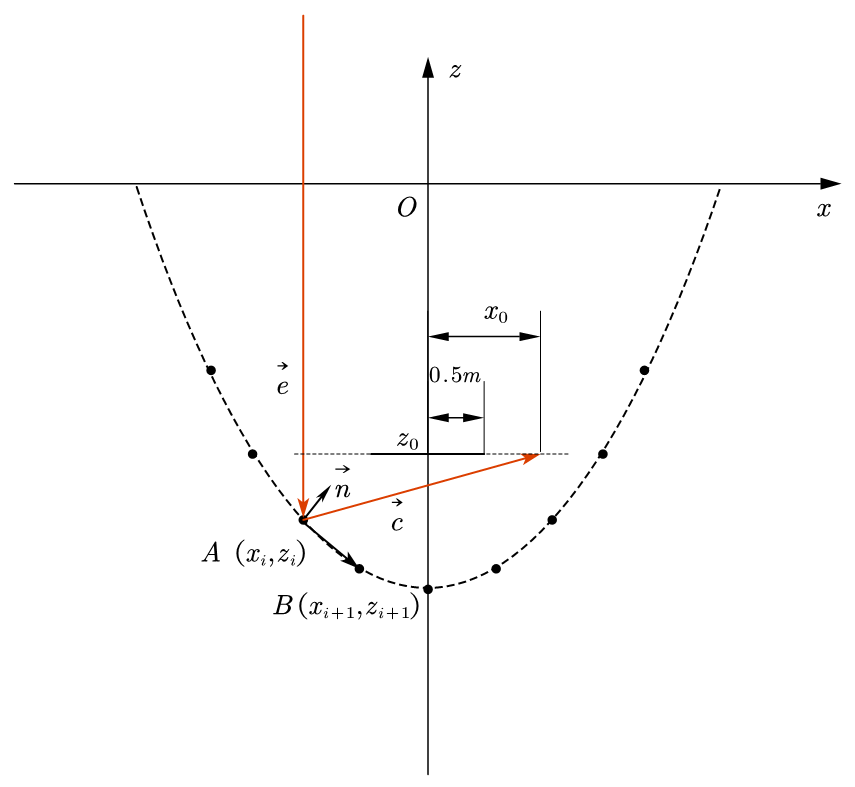
\includegraphics[width=0.6\textwidth]{问题3离散抛物面反射}
		\caption{问题3离散抛物面反射原理}
		\label{问题3离散抛物面反射}
	\end{figure}
	电磁波竖直入射在A点,A点右邻点记为B。入射向量$\overrightarrow{e}$为(0,-1),法向量$\overrightarrow{n}$为:
	\begin{equation}\label{n}
	\overrightarrow{n}=(-\Delta z,\Delta x)=(z_{i}-z_{i+1},x_{i+1}-x_i)
	\end{equation}
	则反射向量$\overrightarrow{c}$为:
	\begin{equation}\label{c}
	\overrightarrow{c}=(c_x,c_z)\overrightarrow{e}-2\left| \overrightarrow{e}\cdot \frac{\overrightarrow{n}}{\left| \overrightarrow{n} \right|} \right|\frac{\overrightarrow{n}}{\left| \overrightarrow{n} \right|}=
	\end{equation}
	反射电磁波的直线方程为:
	\begin{equation}\label{fc}
	z-z_i=\frac{c_z}{c_x}\left( x-x_i \right)
	\end{equation}
	将馈源舱的z坐标$z_0=-(1-0.466)R$代入反射电磁波的直线方程,求得交点的x坐标$x_0$为:
	\begin{equation}\label{x0}
	x_0=\frac{c_x}{c_z}\left( z_0-z_i \right) +x_i
	\end{equation}
	如果$x_0\leqslant 0.5m$,说明反射电磁波被馈源舱接收。遍历每一个散点,统计被接收的比例即可得到xOz截面上的接收比。同理可以求得yOz截面的接收比。按公式(\ref{lb})计算得到整体的接收比。
	
	\subsubsection{抛物面接收比计算结果}
	按上述方法计算xOz截面和yOz截面的接收比,得到xOz截面的接收比$\lambda_1=0.9209$,yOz截面的接收比$\lambda_2=0.9099$,按公式(\ref{lb})计算得到整体的接收比$\lambda=0.8380$。所以馈源舱有效区域接收到的反射 信号 与 3 00 米口径内 反射面 的反射 信号 之比为$83.80\%$。
	
	\subsubsection{基准球面接收比的计算}
	当反射面是基准球面时,从300m口径边缘入射的电磁波一定无法被馈源舱接收,当入射电磁波沿旋转对称轴入射时,则一定能被馈源舱接收。
					\begin{figure}[!htp]
		\centering
		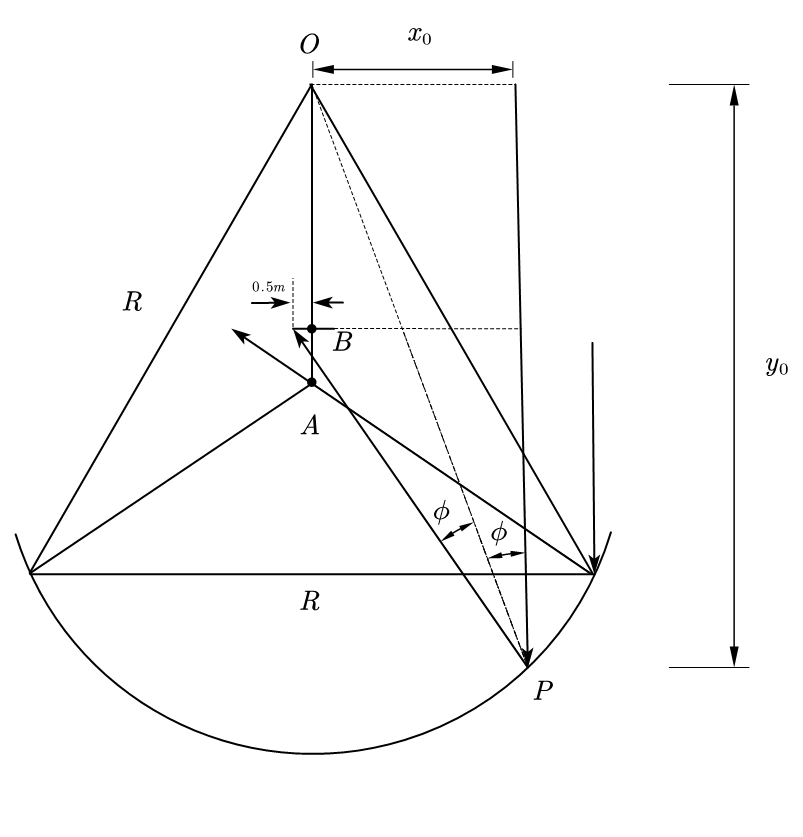
\includegraphics[width=0.6\textwidth]{问题3球面反射示意图}
		\caption{问题3球面反射示意图}
		\label{问题3球面反射示意图}
	\end{figure}

	因此存在一个临界距离,其入射的电磁波经过反射后正好通过馈源舱边缘(半径0.5m),设这个临界距离为$x_0$,入射点纵坐标为$y_0$,则$x_0$和$y_0$满足如下关系:
	\begin{equation}
	\begin{gathered}
	x_{0}{ }^{2}+y_{0}{ }^{2}=R^{2} \\
	\tan \phi=\frac{x_{0}}{y_{0}} \\
	\tan (2 \phi)=\frac{2 \tan \phi}{1-\tan ^{2} \phi}=\frac{0.5+x_{0}}{y_{0}-(1-0.466) R}
	\end{gathered}
	\end{equation}
	解得$x_0=107.8965m$,则基准球面接收比为:
	\begin{equation}
	\left(\frac{x_{0}}{150}\right)^{2}=0.5174
	\end{equation}
	
	\subsubsection{抛物面和基准球面接收比的比较}
	计算得到的抛物面的接收比为$83.80\%$,基准球面接收比为$51.74\%$,相比之下,接收比提高了$61.96\%$。因此把球面调整为抛物面后接收比改善较为显著。
	
	\subsection{灵敏性分析}
	考虑到$h$值的改变会影响到问题2的收敛时误差和最大位移值,以及问题3的的接收比,因此对$h$作灵敏性分析,其中最大位移值随h的改变比例的变化如图\ref{主索点最大径向移动距离随h改变量的变化},收敛时误差随h的改变比例的变化如图
	\begin{figure}[H]
		\centering
		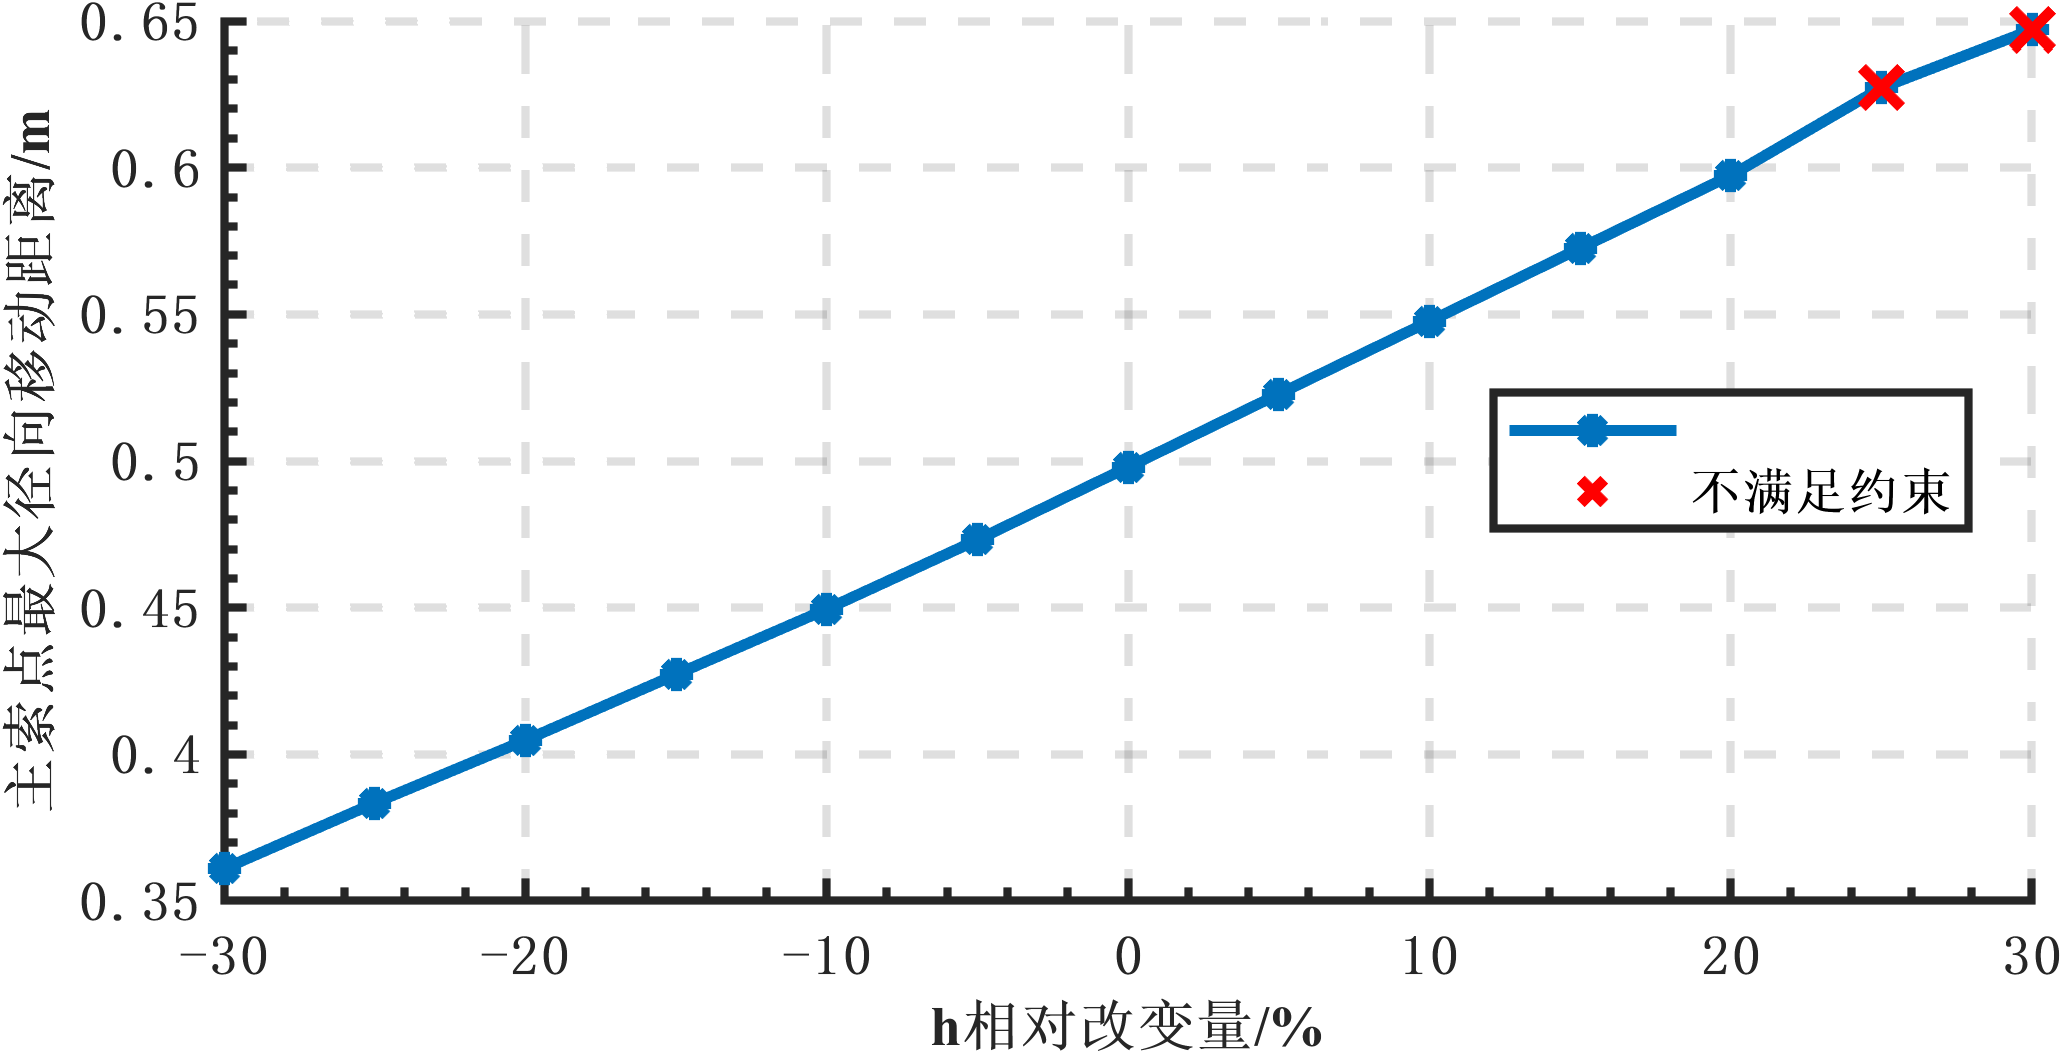
\includegraphics[width=0.6\textwidth]{主索点最大径向移动距离随h改变量的变化}
		\caption{主索点最大径向移动距离随h改变量的变化}
		\label{主索点最大径向移动距离随h改变量的变化}
	\end{figure}
	\begin{figure}[H]
		\centering
		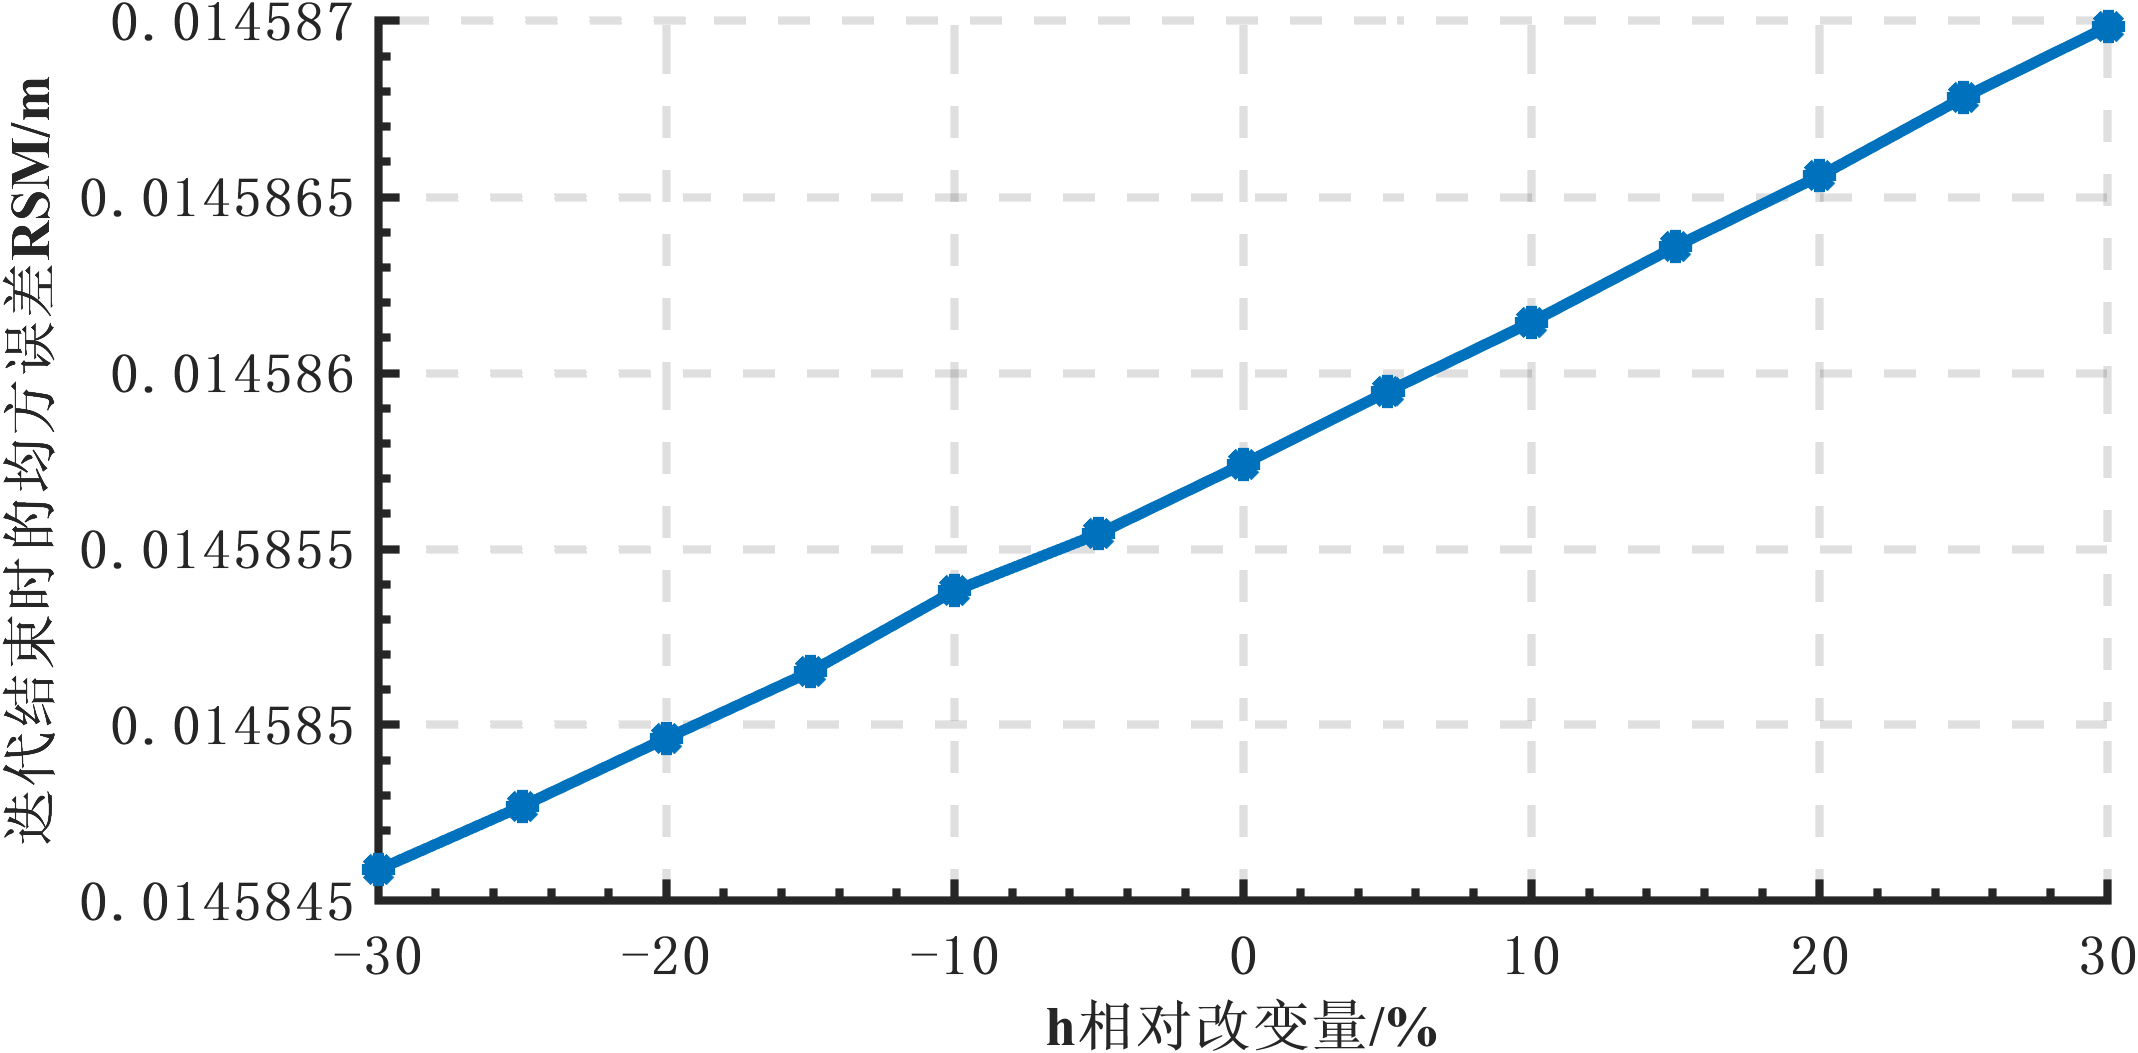
\includegraphics[width=0.6\textwidth]{迭代结束时的均方误差RSM随h改变量的变化}
		\caption{迭代结束时的均方误差RSM随h改变量的变化}
		\label{迭代结束时的均方误差RSM随h改变量的变化}
	\end{figure}
	\begin{figure}[H]
		\centering
		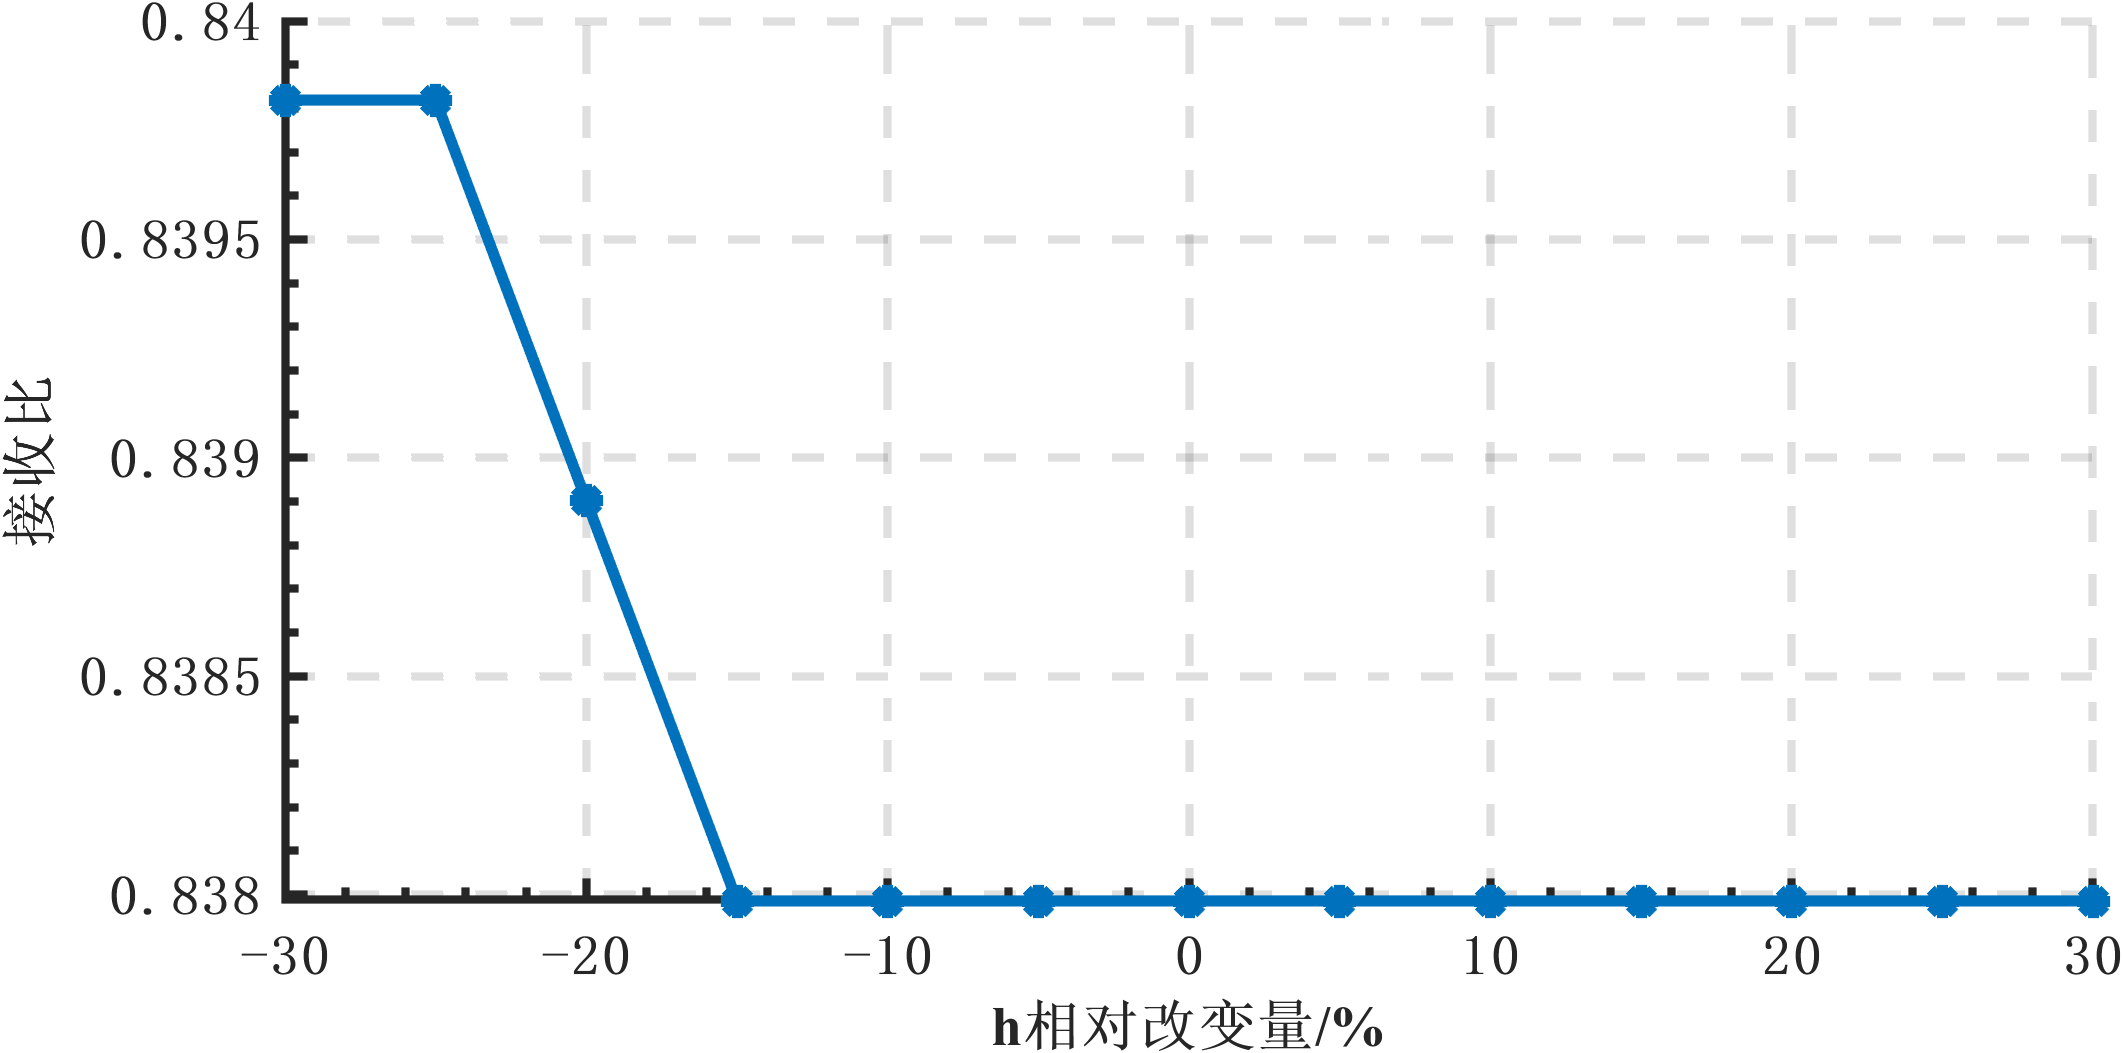
\includegraphics[width=0.6\textwidth]{接收比随h改变量的变化}
		\caption{接收比随h改变量的变化}
		\label{接收比随h改变量的变化}
	\end{figure}
	可以看出,迭代结束时的均方误差RSM和接收比基本不变,$h$对主索点最大径向移动改变影响较大,这是显然的。

	
	
	\section{模型的评价}
\subsection{模型的优点}
\begin{itemize}
	\item 模型建立过程中,运用建立极坐标与旋转坐标系等操作,简化了计算形式,计算过程更加清晰。
	\item 问题二求解节点移动的模型中,对各节点单独进行分析求解,以达到全局最优,迭代次数少计算速度快,且不会由于随即性进入局部最优解。
	\item 问题三中对节点进行平滑插值,简化计算量的同时,兼顾了平面内部点的反射情况。
\end{itemize}
\subsection{模型的缺点}
\begin{itemize}
	\item 模型将反射面近似为平面,与实际情况并不完全一致,存在误差。
	\item 问题二求解过程中没有考虑部分处于理想抛物面的反射面的情况,遗漏了少量拟合点的计算。
	\item 问题三中平面截取次数不够充分,接受比计算精度仍可提升。
\end{itemize}
	
	%参考文献
	%	\begin{thebibliography}{9}%宽度9
	%		\bibitem[1]{liuhaiyang2013latex}
	%		刘海洋.
	%		\newblock \LaTeX {}入门\allowbreak[J].
	%		\newblock 电子工业出版社, 北京, 2013.
	%		\bibitem[2]{mathematical-modeling}
	%		全国大学生数学建模竞赛论文格式规范 (2020 年 8 月 25 日修改).
	%		\bibitem{3} \url{https://www.latexstudio.net}
	%	\end{thebibliography}
	
	%\section{参考文献}
	%\addcontentsline{toc}{section}{参考文献}
	%\bibliographystyle{bib/gbt7714-2005}
	\nocite{*}
	\bibliographystyle{gbt7714-numerical}
	%\bibliographystyle{unsrt}
	%\bibliographystyle{IEEEtran}
	\bibliography{bib/ref.bib}
	
	\newpage
	%附录
	\begin{appendices}
		\section{文件列表}
		% Table generated by Excel2LaTeX from sheet 'Sheet1'
		\begin{table}[htbp]
			\centering
			\caption{Add caption}
			\begin{tabularx}{\textwidth}{@{}c *1{>{\centering\arraybackslash}X}@{}}
				\toprule[1.5pt]
				文件名   & 文件描述 \\
				\midrule
				Data1.mat & 附件1数据 \\
				Data2.mat & 附件2数据 \\
				Data3.mat & 附件3数据 \\
				problem1.m & 问题1求解h \\
				problem2\_1.m & 问题1求解h \\
				problem2\_2.m & 问题2求解其他要求的数据 \\
				problem3.m & 问题3求解抛物面接收比 \\
				solvex0.m & 问题3球面接收比求解 \\
				linminxin.m & 灵敏性分析 \\
				huangjin.m & 黄金分割法 \\
				result.xlsx & 问题二结果表格 \\
				\bottomrule
			\end{tabularx}%
			\label{tab:addlabel}%
		\end{table}%
		
		\section{代码}
				problem1.m
		\lstinputlisting[language=matlab]{code/problem1.m}
		problem2\_1.m
		\lstinputlisting[language=matlab]{code/problem2_1.m}
		problem2\_2.m
		\lstinputlisting[language=matlab]{code/problem2_2.m}
		problem3.m
		\lstinputlisting[language=matlab]{code/problem3.m}
		solvex0.m
		\lstinputlisting[language=matlab]{code/solvex0.m}
		problem3.m
		\lstinputlisting[language=matlab]{code/problem3.m}
		linminxin.m
		\lstinputlisting[language=matlab]{code/linminxin.m}
		huangjin.m
		\lstinputlisting[language=matlab]{code/huangjin.m}
	\end{appendices}
	
\end{document} 